\documentclass[a4paper, 12pt]{article}

\usepackage{inputenc}
\usepackage[british,UKenglish]{babel}
\usepackage{amsmath}
%\usepackage{titlesec}
\usepackage{color}
\usepackage{graphicx}
\usepackage{fancyref}
\usepackage{hyperref}
\usepackage{float}
\usepackage{scrextend}
\usepackage{setspace}
\usepackage{xargs}
\usepackage{multicol}
\usepackage{nameref}

\usepackage{sectsty}
\usepackage{multicol}
\usepackage{multirow}
\usepackage[procnames]{listings}
\usepackage{appendix}
\usepackage{geometry}
\usepackage{titlesec}

\newcommand\tab[1][1cm]{\hspace*{#1}}
\hypersetup{colorlinks=true, linkcolor=black}
\interfootnotelinepenalty=10000

\newcommand{\cleancode}[1]{\begin{addmargin}[3em]{3em}\texttt{\textcolor{cleanOrange}{#1}}\end{addmargin}}
\newcommand{\cleanstyle}[1]{\text{\textcolor{cleanOrange}{\texttt{#1}}}}


\usepackage[colorinlistoftodos,prependcaption,textsize=footnotesize]{todonotes}
\newcommandx{\commred}[2][1=]{\textcolor{Red}
{\todo[linecolor=red,backgroundcolor=red!25,bordercolor=red,#1]{#2}}}
\newcommandx{\commblue}[2][1=]{\textcolor{Blue}
{\todo[linecolor=blue,backgroundcolor=blue!25,bordercolor=blue,#1]{#2}}}
\newcommandx{\commgreen}[2][1=]{\textcolor{OliveGreen}{\todo[linecolor=OliveGreen,backgroundcolor=OliveGreen!25,bordercolor=OliveGreen,#1]{#2}}}
\newcommandx{\commpurp}[2][1=]{\textcolor{Plum}{\todo[linecolor=Plum,backgroundcolor=Plum!25,bordercolor=Plum,#1]{#2}}}

\def\code#1{{\tt #1}}

\def\note#1{\noindent{\bf [Note: #1]}}

\makeatletter
%% The "\@seccntformat" command is an auxiliary command
%% (see pp. 26f. of 'The LaTeX Companion,' 2nd. ed.)
\def\@seccntformat#1{\@ifundefined{#1@cntformat}%
   {\csname the#1\endcsname\quad}  % default
   {\csname #1@cntformat\endcsname}% enable individual control
}
\let\oldappendix\appendix %% save current definition of \appendix
\renewcommand\appendix{%
    \oldappendix
    \newcommand{\section@cntformat}{\appendixname~\thesection\quad}
}
\makeatother


% "define" Scala
\usepackage[T1]{fontenc}  
\usepackage[scaled=0.82]{beramono}  
\usepackage{microtype} 

\sbox0{\small\ttfamily A}
\edef\mybasewidth{\the\wd0 }

\lstdefinelanguage{scala}{
  morekeywords={abstract,case,catch,class,def,%
    do,else,extends,false,final,finally,%
    for,if,implicit,import,match,mixin,%
    new,null,object,override,package,%
    private,protected,requires,return,sealed,%
    super,this,throw,trait,true,try,%
    type,val,var,while,with,yield},
  sensitive=true,
  morecomment=[l]{//},
  morecomment=[n]{/*}{*/},
  morestring=[b]",
  morestring=[b]',
  morestring=[b]"""
}

\usepackage{color}
\definecolor{dkgreen}{rgb}{0,0.6,0}
\definecolor{gray}{rgb}{0.5,0.5,0.5}
\definecolor{mauve}{rgb}{0.58,0,0.82}

% Default settings for code listings
\lstset{frame=tb,
  language=scala,
  aboveskip=3mm,
  belowskip=3mm,
  showstringspaces=false,
  columns=fixed, % basewidth=\mybasewidth,
  basicstyle={\small\ttfamily},
  numbers=none,
  numberstyle=\footnotesize\color{gray},
  % identifierstyle=\color{red},
  keywordstyle=\color{blue},
  commentstyle=\color{dkgreen},
  stringstyle=\color{mauve},
  frame=single,
  breaklines=true,
  breakatwhitespace=true,
  procnamekeys={def, val, var, class, trait, object, extends},
  procnamestyle=\ttfamily\color{red},
  tabsize=2
}

\lstnewenvironment{scala}[1][]
{\lstset{language=scala,#1}}
{}
\lstnewenvironment{cpp}[1][]
{\lstset{language=C++,#1}}
{}
\lstnewenvironment{bash}[1][]
{\lstset{language=bash,#1}}
{}
\lstnewenvironment{verilog}[1][]
{\lstset{language=verilog,#1}}
{}



\lstset{frame=, basicstyle={\footnotesize\ttfamily}}
\geometry{left=3.17cm,right=3.17cm,top=2.54cm,bottom=2.54cm}
% 常规页眉页脚
\newpagestyle{main}{            
    \sethead{}{年度报告}{}     %设置页眉
    \setfoot{}{\thepage}{}      %设置页脚,可以在页脚添加 \thepage  显示页数
    \headrule                                      % 添加页眉的下划线
    \footrule                                       %添加页脚的下划线
}

% 封面页眉页脚
\newpagestyle{title}{            
    \sethead{报告号: 774323540--10dz1200500/01}{}{}     %设置页眉
%    \setfoot{左页脚}{\thepage}{右页脚}      %设置页脚,可以在页脚添加 \thepage  显示页数
    \headrule                                      % 添加页眉的下划线
    \footrule                                       %添加页脚的下划线
}

\pagestyle{main}

\graphicspath{ {images/} }
\usepackage{ctex}
\usepackage{caption}
\usepackage{subfigure}
\usepackage{booktabs}
\usepackage{amsthm}
\usepackage[nottoc]{tocbibind}

\theoremstyle{definition}
\newtheorem{definition}{Definition}[section]
\newtheorem{lemma}{Lemma}
%-----------------------------------------BEGIN DOC----------------------------------------

\begin{document}
\renewcommand{\contentsname}{\ \ \ 目录\ \ \ }
\renewcommand{\appendixname}{附录}
\renewcommand{\appendixpagename}{附录}
\renewcommand{\refname}{参考文献} 
\renewcommand{\figurename}{图}
\renewcommand{\tablename}{表}
\renewcommand{\today}{\number\year 年 \number\month 月 \number\day 日}

\renewcommand{\maketitle}{
    \thispagestyle{title}
    \songti %set font for title
    \vspace*{94pt}
    \begin{center}
        \fontsize{50pt}{0} 科技报告\\
        \vspace*{300pt}
        \large \textcolor{red}{项目名称: \quad}\ \ \underline{\makebox[300pt]{待填写}}\\
        \large 课题名称: \quad\ \ \underline{\makebox[300pt]{待填写}}\\
        \large 编制单位: \quad\ \ \underline{\makebox[300pt]{待填写}}\\
        \large 编制时间: \quad\ \ \underline{\makebox[300pt]{\today}}

    \end{center}
}

\maketitle


\songti %set font for text
\newpage

%-----------------------------------------ABSTRACT-------------------------------------
\begin{center}
{\Large\bf{摘\ 要\\}}
\end{center}
请在这里输入摘要内容.
\newpage
%-----------------------------------------ABSTRACT-------------------------------------
\begin{center}
{\Large\bf{版\ 权\ 声\ 明\\}}
\end{center}
该文件受《中华人名共和国著作权法》的保护。ERCESI实验室保留拒绝授权违法复制该文件的权利。任何收存和保管本文件各种版本的单位和个人,未经ERCESI实验室(西北工业大学)同意,不得将本文档转借他人,亦不得随意复制、抄录、拍照或以任何方式传播。 否则,引起有碍著作权之问题,将可能承担法律责任。\newpage
%-----------------------------------------CONTENT-------------------------------------
\begin{center}
\tableofcontents\label{c}
\end{center}
\newpage

%------------------------------------------TEXT--------------------------------------------

%----------------------------------------OVERVIEW-----------------------------------------

\section{微服务动态更新}
\subsection{技术背景}\label{Background}

\subsubsection{研究背景}
随着软件系统规模的扩大,系统维护和演化也变得越来越复杂。传统的应用程序将所有功能都打包成一个独立的单元,因此也被称为单体应用。单体应用架构简单,在开发、测试和部署等方面都比较方便。但随着软件应用的发展,单体应用的弊端开始显现:不够灵活,对应用程序做任何细微的修改都需要将整个应用程序重新构建、重新部署,妨碍软件应用的持续交付;技术栈受限,开发团队的所有成员通常都必须使用相同的开发语言。因此,微服务架构应运而生。微服务架构将大型的单体应用拆分成若干个更小的服务,使得每个服务都可以独立地进行部署、升级、扩展和替换,服务间使用轻量级的通信协议进行通信(例如,同步的REST,异步的AMQP等),降低服务间耦合度的同时满足了软件程序对于快速持续集成和持续交付的需求。
\begin{figure}[ht]
 \centering
 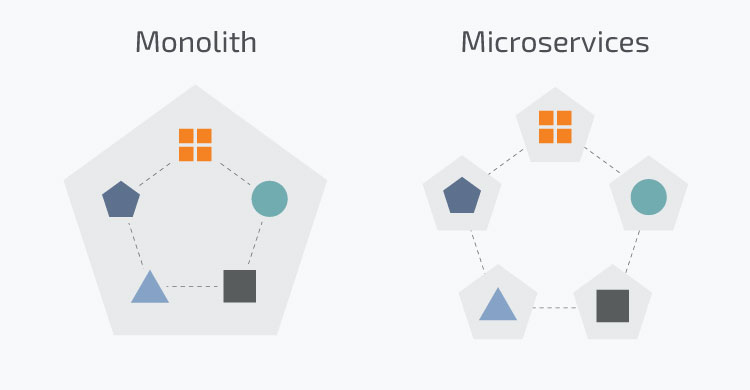
\includegraphics[height=5cm]{images/Microservices-vs-Monolith.jpg}
 \caption{单体应用和微服务应用}
 \label{fig:Microservices-vs-Monolith}
\end{figure}

微服务可以帮助我们对应用进行有效地拆分,缩短软件开发周期,降低软件维护成本。但随着用户需求和软件运行环境的不断变化,已经部署的软件需要不断进行更新修复,以扩展整个系统的功能,提高软件的性能,或者是修复软件存在的故障缺陷。然而,随着用户越来越依赖于系统,他们越来越不能接受传统的停止,更新,重启的软件更新方式。因为直观来说,系统中断会给用户带来不便,引起管理代价的显著提高,比如一些高可靠服务的平台会因为服务中断而蒙受名誉和经济的损失,如云服务平台、银行交易系统。因此我们需要在不中断软件正常运行的前提之下,对软件系统进行更新,即动态软件更新(dynamic software update)。具体来讲,动态软件更新(也称动态适应(dynamic adaption)、运行时更新(run-time update)、动态演化(dynamic evolution))是指软件在运行过程中,不停止已有应用的执行,而实现的运行时行为变更。

软件的动态更新并不容易实现,在安全性、及时性、低干扰性方面面临着巨大的挑战。安全性保证应用程序在更新过程中及更新过程后均能正确运行。及时性要求动态更新操作能够尽快完成,从而减少动态更新影响的持续时间。低干扰性要求更新过程尽量减少对用户影响的程度,提升用户体验。

\subsubsection{相关技术}
微服务架构的一大特点就是不同的服务间可以独立分布式地进行部署,常见的微服务更新部署方式有:
\begin{itemize}
	\item{蓝绿部署(Blue/Green Deployment)

	蓝绿部署是一种基于硬件的动态更新技术,关键在于使用冗余的硬件设备,即在保持当前系统正常运行的前提下,在额外的一台机器上加载新的软件系统,测试完成之后,将流量切到新版本的系统上,这样的动态更新方式在安全性,及时性上没有太大的问题,但是在更新时,会阻断用户正在进行的业务,存在一定的干扰性,且成本较大,需要准备两套}
	\begin{figure}[ht]
	 \centering
	 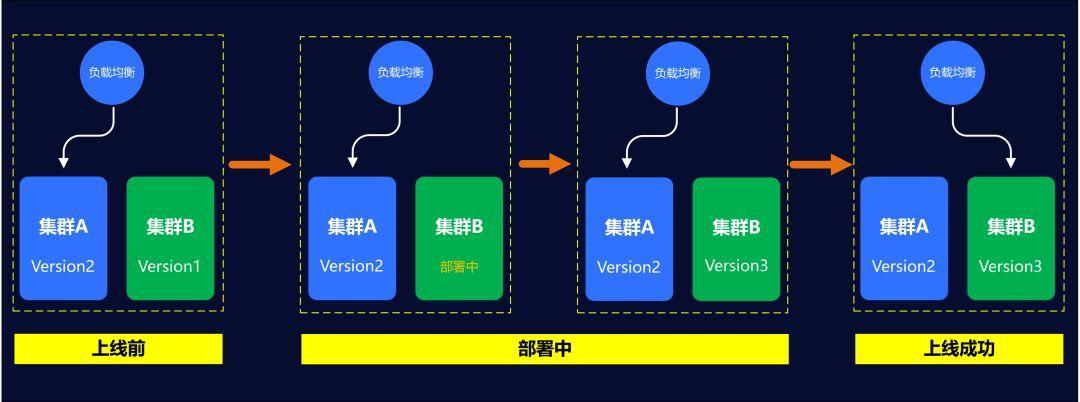
\includegraphics[height=4cm]{images/blue-green.jpeg}
	 \caption{蓝绿部署}
	 \label{fig:blue-green}
	\end{figure}

	\item{灰度发布/金丝雀部署(Canary Update)

	灰度发布是一种软件发布方式,以A/B新旧两个版本为例:让大部分用户继续用老版本A,同时让一小部分用户开始使用新版本B,在部署新版本应用中,需要排掉原有的流量并进行部署。然后根据用户反馈,逐步扩大新版本应用范围,最终实现版本的更新。灰度发布是目前工业界中比较流行的动态更新方式,但是不可避免地会在更新过程中干扰用户正在进行的事务。}
	\begin{figure}[ht]
	 \centering
	 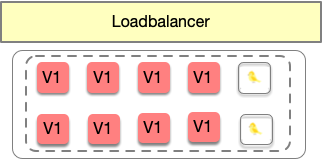
\includegraphics[height=3cm]{images/canary.png}
	 \caption{灰度发布/金丝雀部署}
	 \label{fig:canary}
	\end{figure}

	\item{滚动发布(Rolling Update)

	滚动发布是指取出一个或多个服务器停止服务,执行更新,并重新将其投入使用。周而复始,直到集群中所有的实例都更新成最新版本。这种动态更新方式相较于蓝绿部署,虽然节约了硬件资源,但是会遇到更多的问题,在金丝雀发布基础上的进一步优化改进,是一种自动化程度较高的发布方式。}
	
\end{itemize}
上述的微服务更新部署方式,都保证了更新过程中服务的可用性。但由于更新的时机是任意可选的,用户的请求也是会实时产生的,这样就难免会出现用户某一次请求前一次访问的是旧版本的微服务实例,随后服务进行了更新,本次请求再次调用到的变成了新版本的微服务实例。如新旧版本的服务存在不可兼容性,这样的行为显然将返回错误,也即破坏了动态更新对于安全性的要求。


\newpage
\subsection{微服务动态演化一致性保障协议}\label{section:version_consistency}

\subsubsection{基本原理}
本小节将阐述微服务动态演化一致性保障协议的基本原理,说明如何保证正确且高效地完成系统的动态演化。首先引入一个简单但又不失一般性的例子,在系统中存在着这样四个微服务:Portal、Proc、Auth和DB。用户首先会向Portal微服务发起请求,收到请求后的Portal微服务先是调用Auth微服务,得到当前请求的一个验证令牌。然后Portal使用得到的令牌接着对Proc微服务发起请求,收到请求的Proc微服务利用随请求而来的令牌向Auth微服务进行验证,若收到的回复是验证通过,则进一步调用DB微服务以读取数据库中的具体信息并返回;否则,返回请求失败消息,然后将最终结果反馈给发起请求的用户。
\begin{figure}[ht]
 \centering
 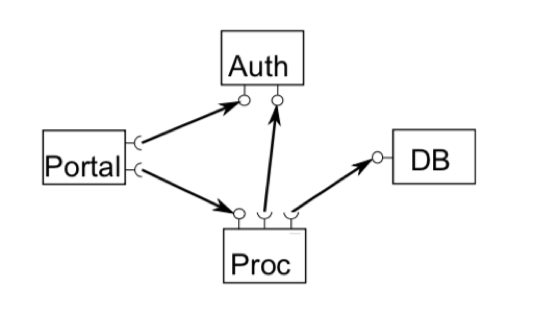
\includegraphics[height=5cm]{images/Example.png}
 \caption{示例系统}
 \label{fig:Example}
\end{figure}


考虑到这样一种情况:在系统运行时,由于采用了更为安全和快速的加解密算法,由于整个系统所有的加解密过程都在Auth微服务中进行,因此我们可以仅对Auth微服务进行版本的更新及替换,同时对其它的微服务保持透明。在前述的系统运行流程中,若我们在Portal微服务调用完Auth微服务得到对应的验证令牌后且Proc微服务还未使用该令牌向Auth微服务发起验证之前的这个时间段内,Auth微服务不服务于任何的事务,处于空闲状态,我们对Auth微服务进行版本的更新及替换。随着系统的继续运行,当Proc微服务利用使用旧版本算法所加密生成的验证令牌来向Auth微服务发起调用,但此时的Auth微服务已完成更新,新旧算法的不兼容性导致验证失败,最终返回失败信息。显然Auth微服务不正确的动态演化,导致了系统在无故障的情况下不能正确地处理用户请求。

动态演化要求系统能够在不停止服务的情况下进行更新,用户发出的请求在更新前后都能被正确地处理且返回结果。因此,微服务动态演化一致性保障协议的基本原理是考虑在系统运行的过程中,当一次请求需要多次涉及同一个微服务,且不同版本的微服务因兼容性等原因将返回不同的结果时,需要依据事务的运行流程来决定调用的服务版本,从而保证用户请求不受服务动态演化的影响。

\subsubsection{一致性保障协议}
在介绍一致性保障协议之前,首先介绍协议中将要用到的几个基本概念的定义:

\theoremstyle{definition}
\begin{definition}[\textbf{事务与分布式事务}]
\label{definition:transaction}
\textbf{一个事务表示在某一微服务上执行且在有限时间内结束的一系列操作,操作包括本地数据的计算和微服务间消息的传递等。在某一微服务上运行的事务可以向其它微服务发起请求,从而在其它的微服务中生成一个新的事务。前者和后者之间的事务关系我们称为父子事务,外界调用系统所产生的第一个事务为根事务。根事务及其随后的调用所产生的所有子事务,我们称为一个分布式事务,并使用其根事务的符号进行标识。}
\end{definition}

\begin{figure}[ht]
 \centering
 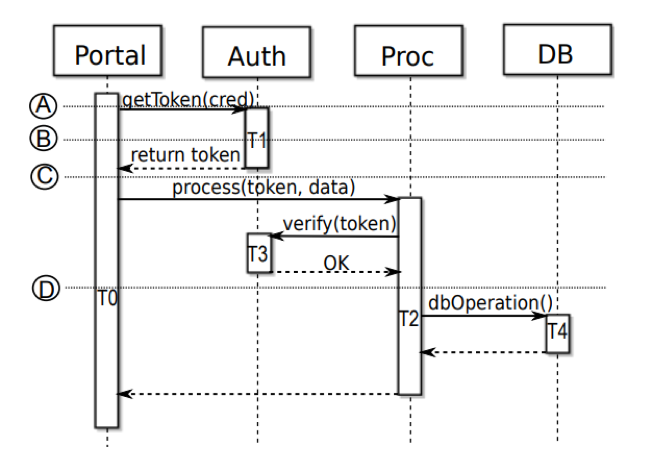
\includegraphics[height=8cm]{images/ExampleProcess.png}
 \caption{示例系统运行时序图}
 \label{fig:ExampleProcess}
\end{figure}


上图即表示了我们前面所描述的系统中四个微服务之间的运行流程。外部请求首先在Portal微服务上生成T0根事务,然后通过微服务间的调用T1、T2、T3、T4事务依次生成。这样一次完整的调用过程我们便称为分布式事务,用根事务符号T0来进行表示,而T1~T4事务都可称为是T0的子事务。

\begin{definition}[\textbf{版本一致性}]
\label{definition:version_consistency}
\textbf{一个分布式事务是版本一致的,当且仅当不存在它的两个子事务,它们在系统运行时先后在同一个微服务的不同版本上运行。一次动态演化所导致的系统演化是版本一致的,当且仅当所有的分布式事务是版本一致的。}
\end{definition}



在我们前面所描述的系统运行的例子中,考虑对Auth微服务进行更新,如果更新发生在根事务T0生成之后,但在生成T1之前(即时刻A),那么后续在Auth微服务上生成的T1、T3子事务都使用的是Auth微服务的新版本,分布式事务T0满足版本一致性;如果更新发生在T3子事务完成之后(即时刻D),那么在Auth微服务执行过的T1、T3子事务都使用的是Auth微服务的旧版本,分布式事务T0满足版本一致性;而在前面系统出现错误的例子中,更新发生在子事务T1完成之后, 但T2子事务还未生成之前(即时刻C),那么将导致T1子事务和T3子事务在Auth微服务的不同版本上运行,此时分布式事务T0便不满足版本一致性。

版本一致性虽然描述了微服务动态演化的准则,但我们并不能直接利用这个规则来对微服务动态演化的时机进行判断,因此我们需要引入动态依赖边,使得我们可以分布式地在各自的微服务上进行本地的操作,便可以判断当前微服务是否满足动态演化的条件(即版本一致性)。

\begin{definition}[\textbf{动态依赖边}]
\label{definition:dynamic_dependences}
\textbf{$C \xrightarrow[T]{future(past)}  C'$表示在分布式事务T的运行过程中,有一条从微服务C到微服务$C'$的future(past)边。
其中,future边表示在T之后的运行过程中,微服务C有可能还会在微服务$C'$上生成新的子事务;past边表示在T之前的运行过程中,微服务C已经在微服务$C'$上成功地生成过子事务并返回。}
\end{definition}



有了动态依赖边的定义,我们使用如下的规范性准则,使得依赖边可以在每一个分布式事务的运行过程中动态且正确地进行增加和删除操作:

\begin{itemize}
\item{在微服务C上运行的每一个事务T,开始时添加一对动态依赖边( $C \xrightarrow[root(T)]{future}C$ 和 $C \xrightarrow[root(T)]{past}C$ ),标识为T的根事务,事务结束时删除;}


\item{每一条动态依赖边,都需要微服务C和微服务$C'$之间存在真正的静态边,即存在对应调用关系;}


\item{$C \xrightarrow[T]{future}C'$ 边必须要在T的第一个子事务生成之前添加,并且应等到T不会通过微服务C在微服务$C'$上生成子事务时,才能够删除;}


\item{$C \xrightarrow[T]{past}C'$ 边在T的运行过程中,当微服务C在微服务$C'$上生成的子事务即将结束时生成,应等到T结束时才能够删除。}
\end{itemize}

有了上述动态依赖边的支持,在系统运行的任何时刻,每个微服务都可以知晓指向自己的动态依赖边,以及负责从自己指向其它微服务动态依赖边的增删,所以我们可以将动态演化的版本一致性条件转化为本地可判断的闲置(FREENESS)条件:

\begin{definition}[\textbf{闲置(FREENESS)}]
\label{definition:freeness}
\textbf{微服务C针对某一个分布式事务T是版本一致的,当且仅当不存在由T标识的一对future/past边指向微服务C。微服务C在某一时刻下的状态是版本一致的,当且仅当微服务C对所有当前运行的分布式事务是版本一致的。}
\end{definition}


\subsubsection{微服务动态演化过程}
利用动态依赖边的定义以及增删的规范性准则,带有动态依赖边的分布式事务T在运行时流程具体表现为如下三个阶段:

\begin{enumerate}

\item [1.] 准备阶段:分布式事务T在第一个微服务C上完成初始化但还未调用任何其它微服务,即生成子事务之前,C通知所有可能依赖的微服务创建future边并等待回复。被通知的微服务同理,通知其依赖的微服务执行创建操作。当收到所有future边创建成功的回复后,事务T开始运行,如图\ref{fig:Process_a};
\begin{figure}[ht]
 \centering
 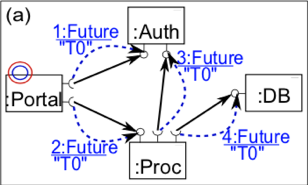
\includegraphics[height=5cm]{images/Process_a.png}
 \caption{准备阶段:process\_a}
 \label{fig:Process_a}
\end{figure}


\item [2.] 运行阶段:当知道微服务C不会再通过静态边 $C \xrightarrow{static}C'$ 在微服务C’上生成T的子事务,而且不存在指向C的标识为T的future边,那么future边 $C \xrightarrow[T]{future}C'$ 可以被删除;当微服务$C'$上标识为T的子事务将要结束时,通知微服务C创建past边 $C \xrightarrow[T]{past}C'$ ,且应保证创建成功才能结束子事务,如图\ref{fig:process_c and process_d};
\begin{figure}[htbp]
\centering
\begin{minipage}[t]{0.48\textwidth}
\centering
\centerline{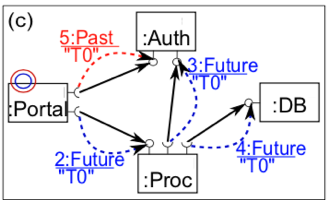
\includegraphics[width=6cm]{Process_c.png}}
\label{fig:process_c}
\end{minipage}
\begin{minipage}[t]{0.48\textwidth}
\centering
\centerline{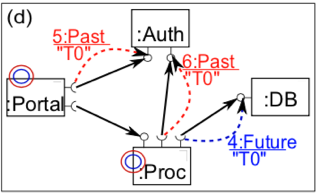
\includegraphics[width=6cm]{Process_d.png}}
\label{fig:process_d}
\end{minipage}
\caption{运行阶段:procss\_c 和 process\_d}
\label{fig:process_c and process_d}
\end{figure}


\item [3.] 结束阶段:和准备阶段时的创建操作类似,从第一个微服务C递归向所有的依赖微服务发送删除消息,删除标识为当前分布式事务T的所有动态依赖边。
\end{enumerate}

前面的运行流程中,假设我们需要对Auth微服务进行一致性演化且当前只有分布式事务T0处于运行状态,利用闲置(FREENESS)的定义,在时刻A和时刻D,Auth满足更新条件;而在时刻C,存在执行Auth微服务且标识为T0的一对future/past边,因此不满足更新条件。

微服务C只有满足了闲置(FREENESS)条件才能够进行动态演化,但由于系统处于持续运行且不断接收请求的状态,同一时刻存在不同的分布式事务在系统中运行,因此若仅仅通过等待然后判断的策略(WF),微服务有可能永远不能满足闲置(FREENESS)条件,从而无法及时地进行动态演化。除了WF策略,我们还可以使用下面的两种策略,使得微服务能够及时地完成动态演化操作:

\begin{itemize}

\item {CV:允许不同版本的微服务实例同时存在并提供服务

当微服务C需要进行动态演化时,启动新版本的实例并同时提供服务。当需要在微服务C上生成子事务T时,若已经有一条标识为root(T)的past边指向微服务C,那么新生成的子事务T将在旧版本的微服务实例上运行,否则在新版本的微服务实例上运行。由于事务会在有限时间内完成,因此旧版本的微服务实例上运行的事务逐渐减少为零,最终将旧版本实例从系统中移除。}

\item{BF:暂时阻塞新事务的生成

当微服务C需要进行动态演化时,若需要在其上生成新的子事务T,首先判断是否存在标识为root(T)的一条past边指向自己,若存在则子事务T可以在微服务C上生成并继续执行;不然,阻塞子事务T。旧版本的微服务实例上运行的事务会在有限时间内完成,最终微服务C将满足闲置(FREENESS)条件,此时进行版本的更新,然后恢复之前阻塞的所有事务。}
\end{itemize}

\newpage
\subsection{基于Istio的协议实现}\label{baseistio}
\subsubsection{Service Mesh与Istio}

与单体应用相比,微服务架构将系统应用的复杂度从单体应用内部的测试、部署、维护等转变到了微服务的连接调用、管理部署和监控等方面,因此微服务架构会极大地增加运维工作量,开发人员需要投入更多的精力来保证远程调用的可靠性与数据一致性。为了简化开发,开发人员通过典型的类库和框架(如Netflix OSS套件、Spring Cloud框架),编写较少的代码和注解就可以完成微服务间的服务发现、负载均衡、熔断、重试等功能。但此种办法缺点在于,开发人员需要掌握并熟练使用的内容较多,而且服务治理的功能不够齐全,很多功能需要自己进行拓展,编程语言也有所受限。

这样所开发出来的微服务中,关键的业务逻辑代码和其它的用于管理服务间关系的非功能性代码混杂在一起。此时,若考虑为每一个微服务实例部署一个Sidecar,将所有前述的非功能性代码移到Sidecar中,由Sidecar来负责提供服务发现等辅助功能,而开发人员只需专注于微服务的业务逻辑,从而有效地进行了解耦。当为大型的微服务系统部署Sidecar时,微服务之间的服务调用关系便形成了服务网格(Service Mesh),如图\ref{fig:service_mesh}所示。
\begin{figure}[ht]
 \centering
 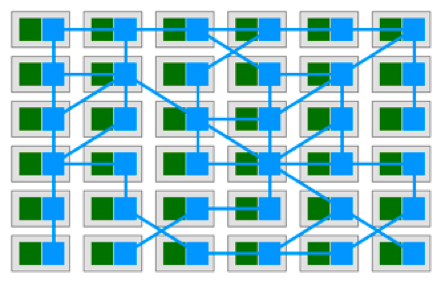
\includegraphics[height=5cm]{images/service_mesh.png}
 \caption{服务网格(Service Mesh)}
 \label{fig:service_mesh}
\end{figure}

当前最主流的Service Mesh方案,是Google和IBM两个公司联合Lyft合作的开源项目Istio。在Istio的架构中,直接在Lyft开发的Envoy之上进行了拓展,然后将其作为Sidecar代理进行部署。Envoy Proxy作为数据面,除了提供服务发现、负载均衡、限流熔断等功能,还可以协调微服务的所有出入站流量,收集相关的性能指标,与控制面进行交互。而有了数据面的支持,控制面一方面通过Pilot组件下发配置信息到相应的Envoy Proxy中,负责流量管理,另一方面通过Mixer组件收集遥测数据,从而实现了对整个微服务系统多方面的掌管与监控。
\begin{figure}[ht]
 \centering
 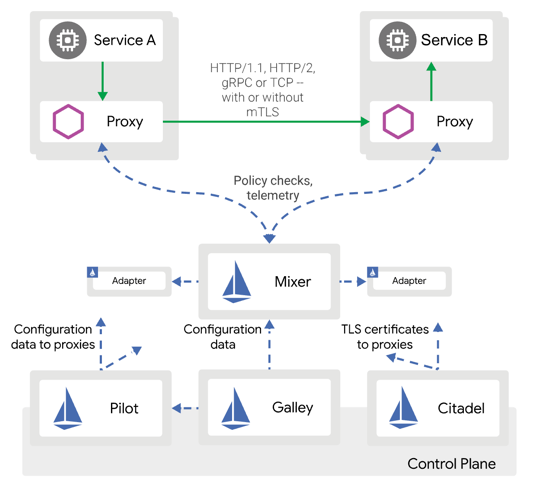
\includegraphics[height=9cm]{images/istio_arch.png}
 \caption{Istio架构图(v1.4)}
 \label{fig:istio_arch}
\end{figure}

\subsubsection{协议实现具体流程}
基于Istio,部署前述的示例系统,具体架构变为图\ref{fig:demo_arch_on_istio}。用户将访问请求发往Ingress Gateway,由Ingress Gateway依据相应的路由规则,再将请求转发至具体的后端服务中,然后收集运行结果并进行返回。每一次用户的请求都将产生一个分布式事务,其中可能会涉及多个服务的远程调用,但可以使用请求头中的x-b3-traceid字段进行唯一标识。Ingress Gaeway一方面将对应的服务接口暴露出来供用户进行访问,另一方面为用户屏蔽了后端服务的具体实现和路由转发等服务治理功能。

\begin{figure}[ht]
 \centering
 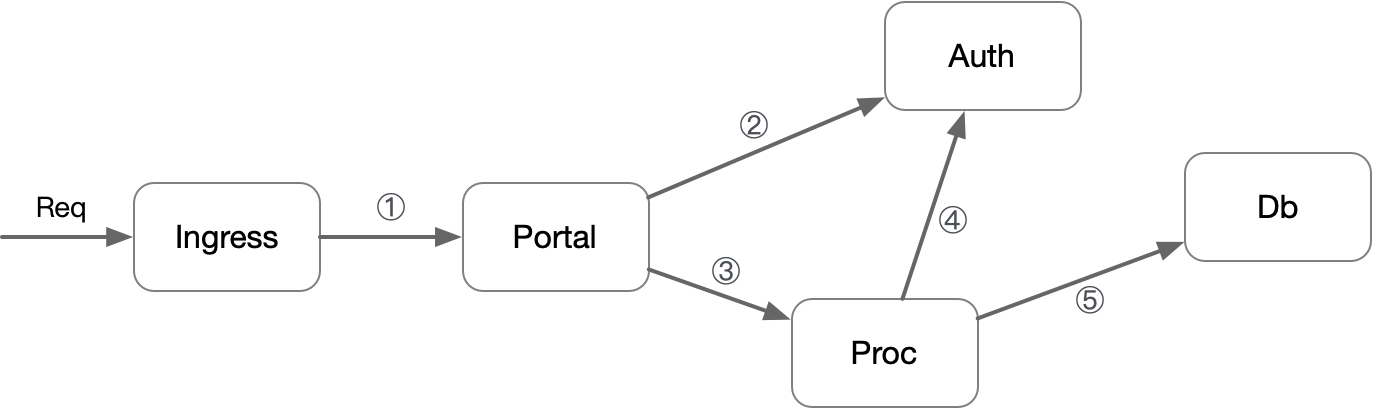
\includegraphics[height=4cm]{images/demo_arch_on_istio.png}
 \caption{Istio中的示例系统}
 \label{fig:demo_arch_on_istio}
\end{figure}

以示例系统中的auth-service服务为例,具体的实现和更新流程为:
\paragraph{插入Envoy容器和TraceManager容器}
修改Istio框架中的自动注入功能,当每个服务实例部署时,我们将为每个服务实例对应部署Envoy容器和TraceManager容器。其中,Envoy容器负责从Istio控制面中接收用户的配置信息,然后将配置信息转换成对应的规则,对所有的出入站流量进行管理;与此同时,当存在具体的入站流量访问对应的服务时,Envoy会将此次分布式调用的唯一标识(x-b3-traceid)和相关信息发送至TraceManager中。而TraceManager容器则负责接收从Envoy容器中发送过来的信息,对其进行记录管理,为后续的更新过程提供支持。插入的Envoy和TraceManager容器分别作为客户端和服务端,通过Unix Domain Socket的方式进行通信,从而最大程度地减少了消息传送对Envoy快速处理用户请求的影响。
\begin{figure}[ht]
 \centering
 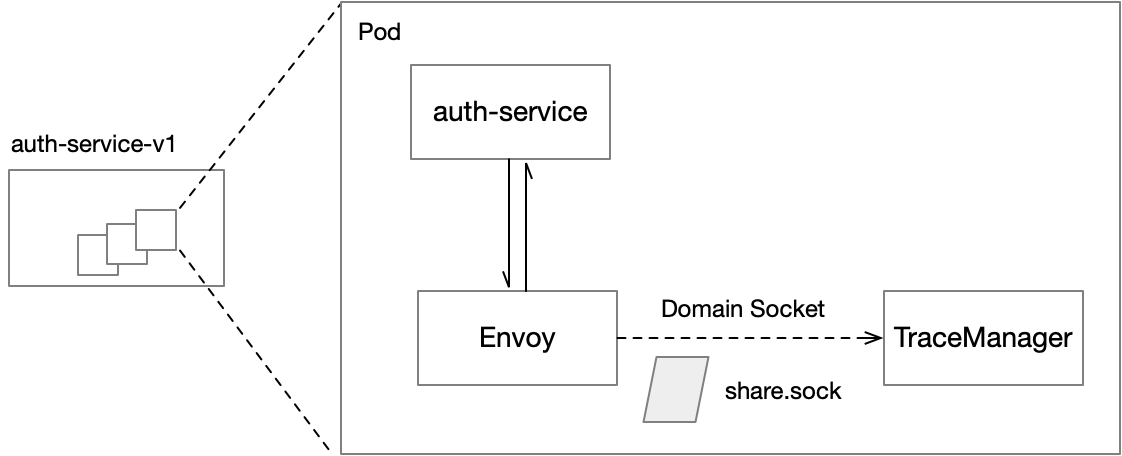
\includegraphics[height=5cm]{images/insert_containers.png}
 \caption{插入容器}
 \label{fig:insert_containers}
\end{figure}

\paragraph{创建初始的路由规则和版本信息}\label{section:setup}当整个系统部署完成时,为每个服务创建初始的路由规则和版本信息。图\ref{fig:vs_all_v1}中定义了路由规则,要求流量调用到auth-service时,所有流量都发往v1版本,且在返回的头信息中会带上自定义的信息,后续将利用此头信息进行流量的转发;图\ref{fig:dr_v1}中定义了版本信息,说明带有{version: v1}标签的所有auth-service的服务实例都属于v1版本;此时系统的运行状态对应显示为图\ref{fig:traffic_all_v1}
\begin{figure}[htbp]
\centering
\begin{minipage}[t]{0.48\textwidth}
\centering
\centerline{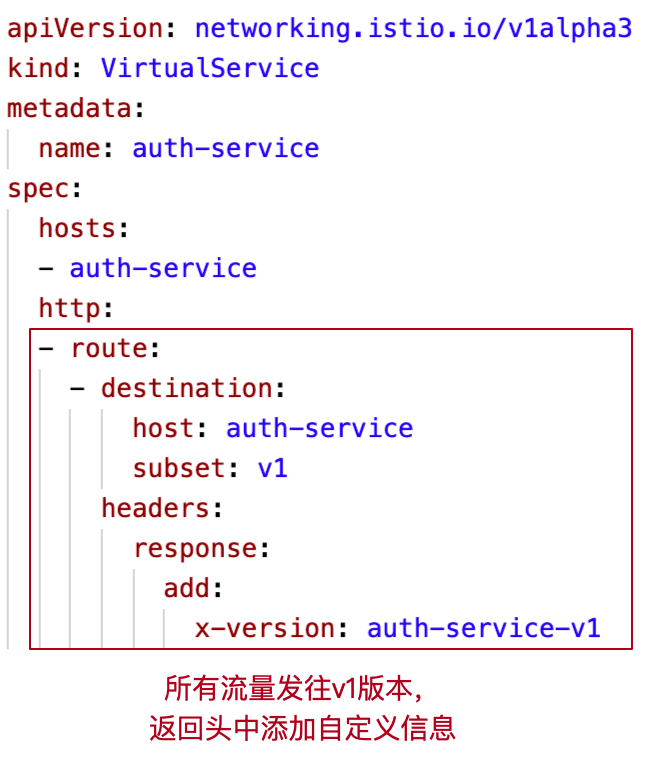
\includegraphics[width=6cm]{vs_all_v1.png}}
\caption{v1路由规则}
\label{fig:vs_all_v1}
\end{minipage}
\begin{minipage}[t]{0.48\textwidth}
\centering
\centerline{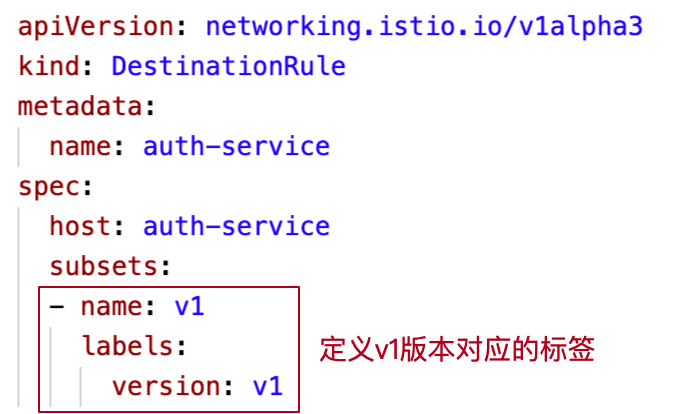
\includegraphics[width=6cm]{dr_v1.png}}
\caption{v1版本规则}
\label{fig:dr_v1}
\end{minipage}
\end{figure}

\begin{figure}[ht]
 \centering
 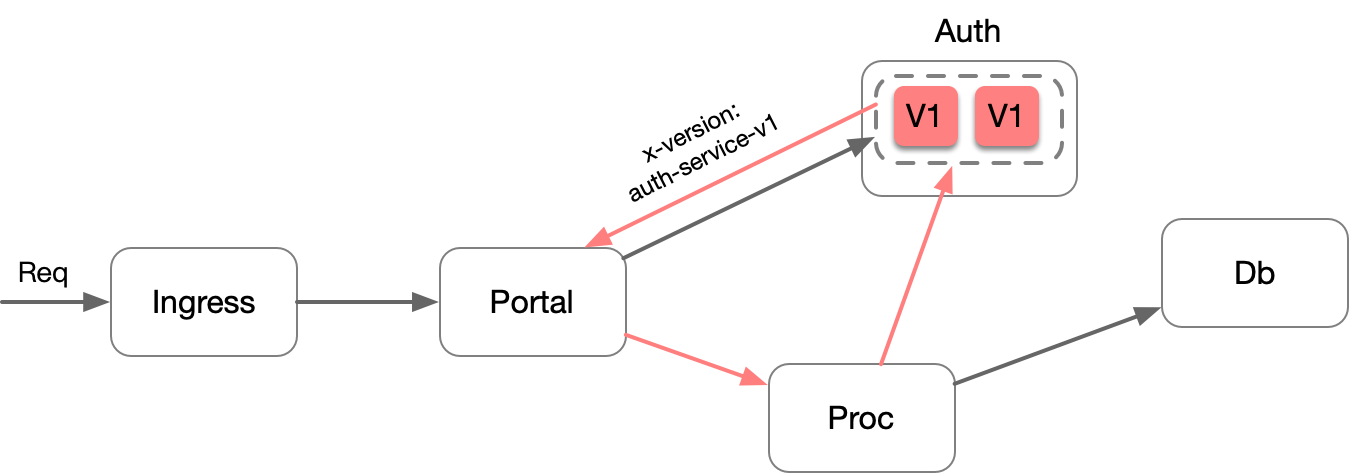
\includegraphics[height=4cm]{images/traffic_all_v1.png}
 \caption{流量全部发往v1}
 \label{fig:traffic_all_v1}
\end{figure}

在系统的运行过程中,当存在入站流量调用到auth-service时,Envoy容器执行拦截操作:一方面将流量转发往负责的服务实例,另一方面将此次调用所对应的traceid信息从头信息中提取出来并发送往TraceManager容器,TraceManager容器则将对应的traceid存到对应的TraceidSet中,该集合代表了当前所有调用过auth-service的分布式事务id;同时,当本次用户请求处理完成并返回Ingress Gateway时,Ingress Gateway实例内部会执行同样的添加操作,这里的TraceidSet则代表了当前已完成并返回的分布式事务id集合。
\begin{figure}[ht]
 \centering
 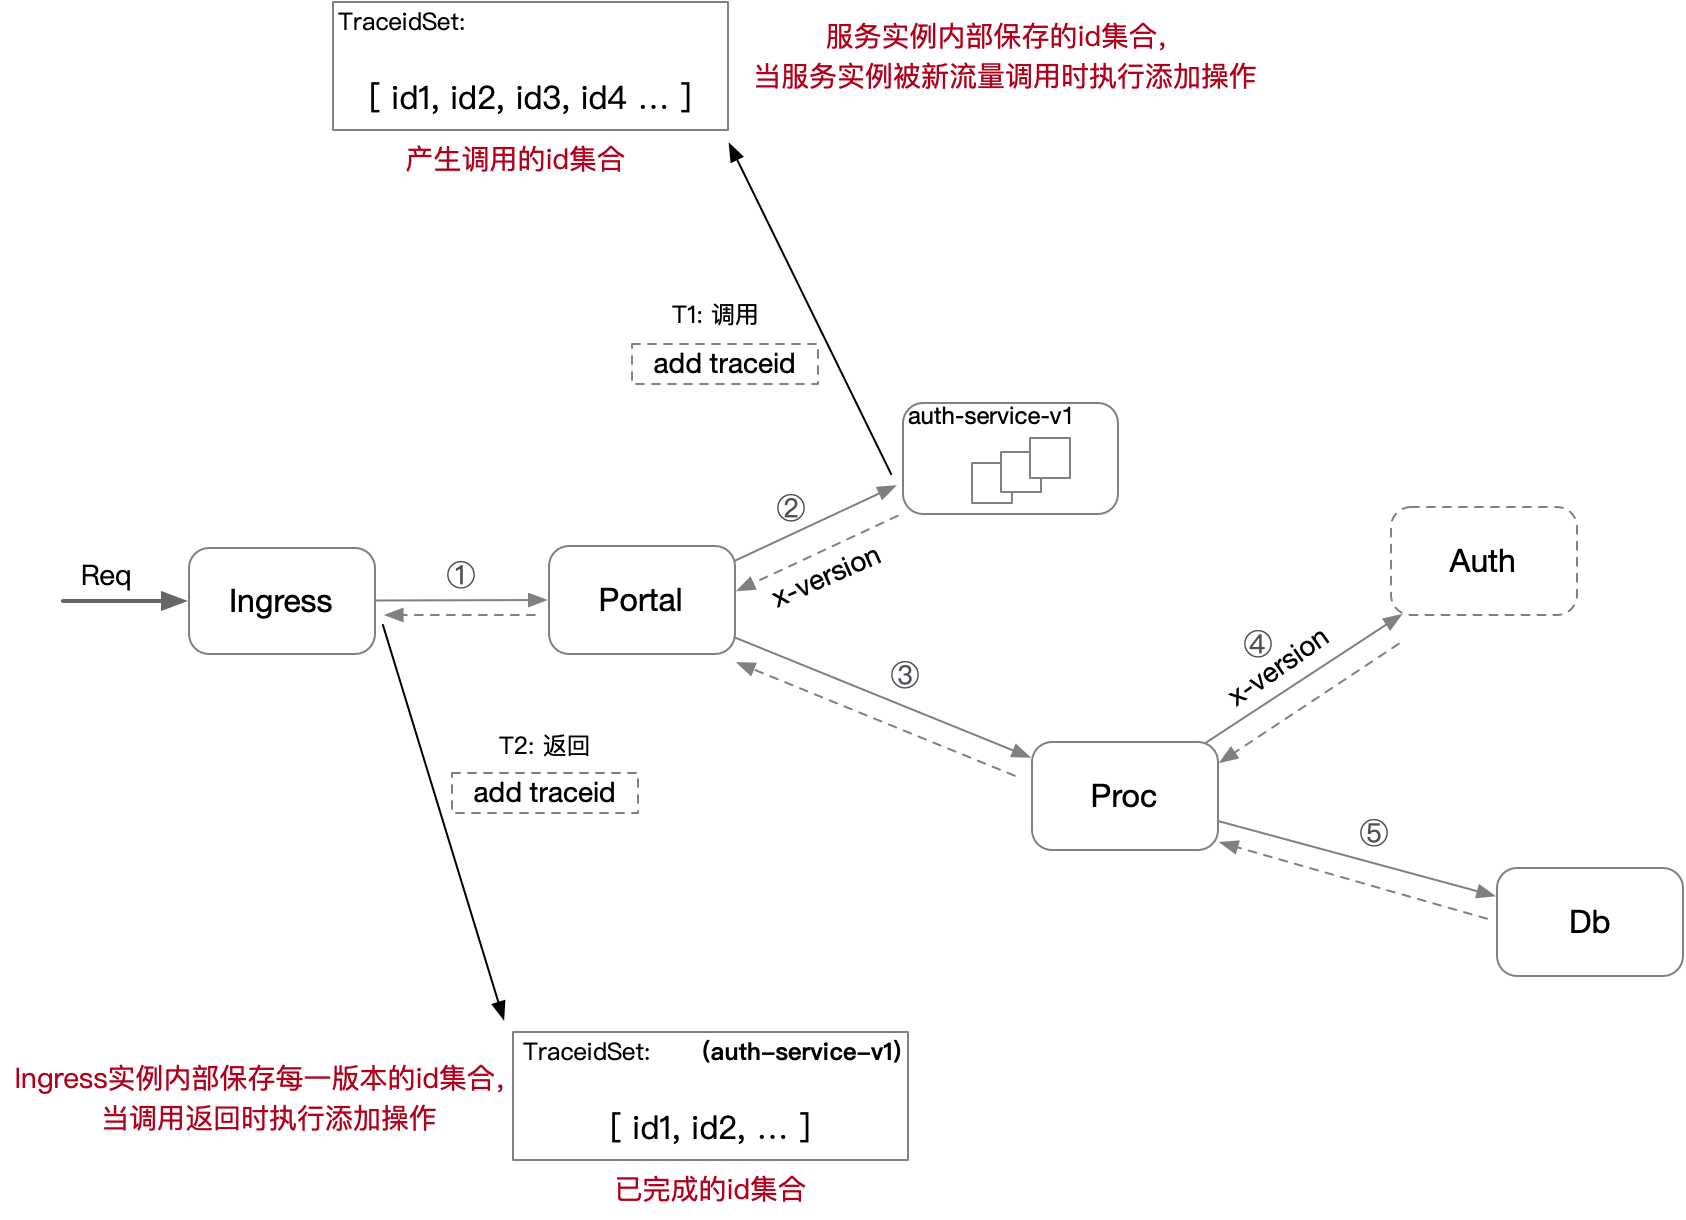
\includegraphics[height=10cm]{images/record_trace.png}
 \caption{事务记录}
 \label{fig:record_trace}
\end{figure}

\paragraph{新版本上线}
当我们需要对auth-service进行更新时,首先需要将新版本的服务进行上线部署。与此同时,相关的路由规则和版本信息修改为:图\ref{fig:vs_default_v1}中共包含三个路由规则,依次进行匹配,第一条规则表示若请求流量中的头信息包含v1版本信息,则将该流量转发到v1版本中;第二条规则表示若请求流量中的头信息包含v2版本信息,则将该流量转发到v2版本中;若第一第二条规则均不满足,则应用第三条规则,将流量转发到v1版本中,同时添加对应的自定义头信息。图\ref{fig:dr_v1v2}则添加了新版本服务对应的标签定义。
\begin{figure}[htbp]
\centering
\begin{minipage}[t]{0.48\textwidth}
\centering
\centerline{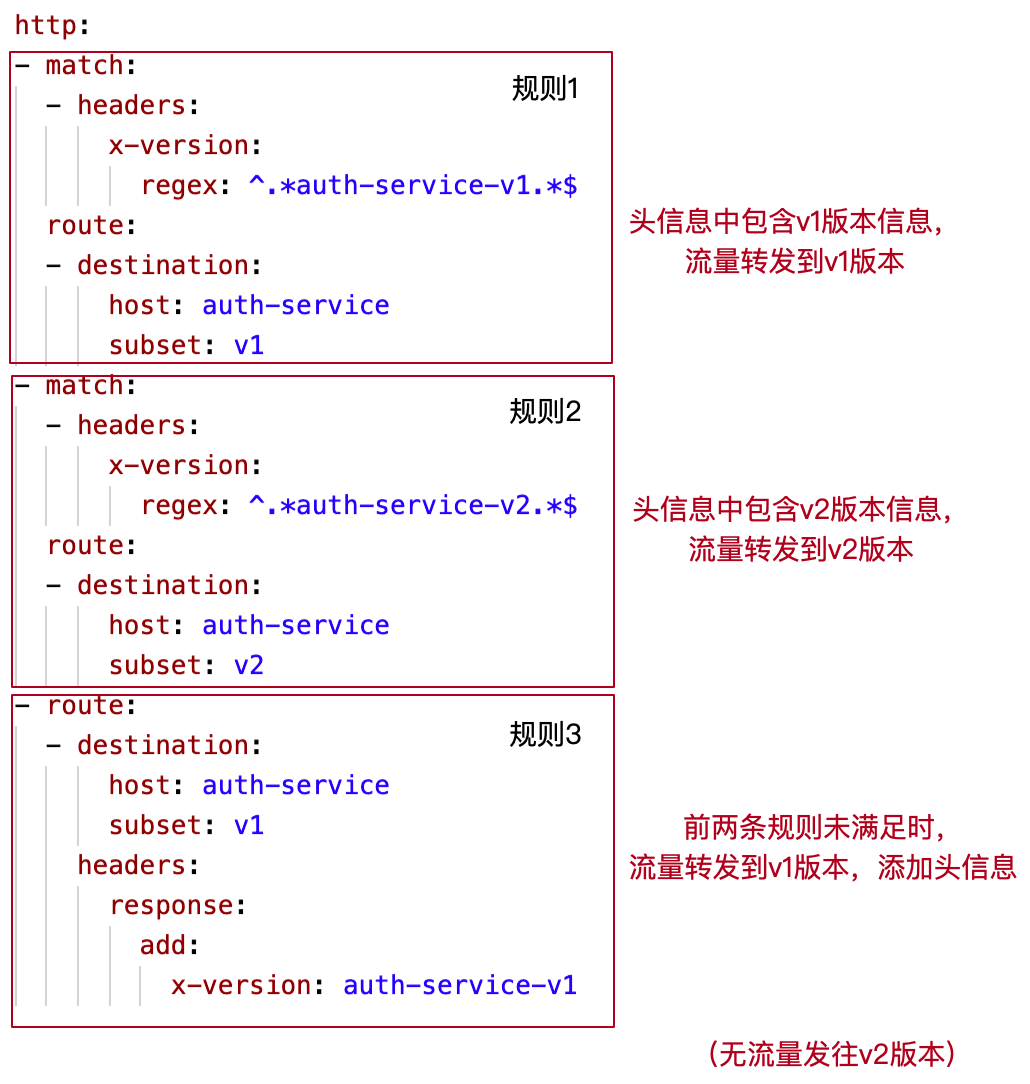
\includegraphics[width=7cm]{vs_default_v1.png}}
\caption{默认发往v1路由规则}
\label{fig:vs_default_v1}
\end{minipage}
\begin{minipage}[t]{0.48\textwidth}
\centering
\centerline{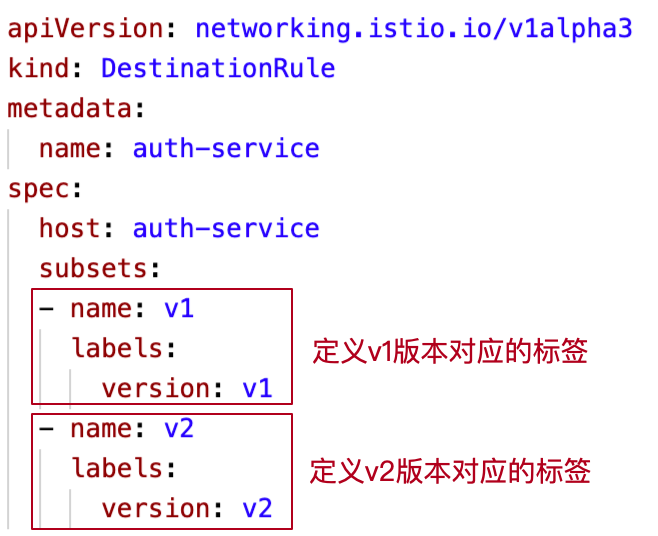
\includegraphics[width=6cm]{dr_v1v2.png}}
\caption{v1、v2版本规则}
\label{fig:dr_v1v2}
\end{minipage}
\end{figure}

此时,若某个分布式事务还未调用过auth-service,则请求的头信息中不包含相关的版本信息,依据第三条规则将流量转发往v1版本;若此分布式事务已调用过auth-service服务,则由于第三条规则的存在,其请求的头信息中必然包含了v1的版本信息,依据第一条规则同样将流量转发往v1版本。因此,虽然新版本的auth-service已完成上线部署,但还没有流量经过。对应的系统运行状态如图\ref{fig:traffic_default_v1}所示
\begin{figure}[ht]
 \centering
 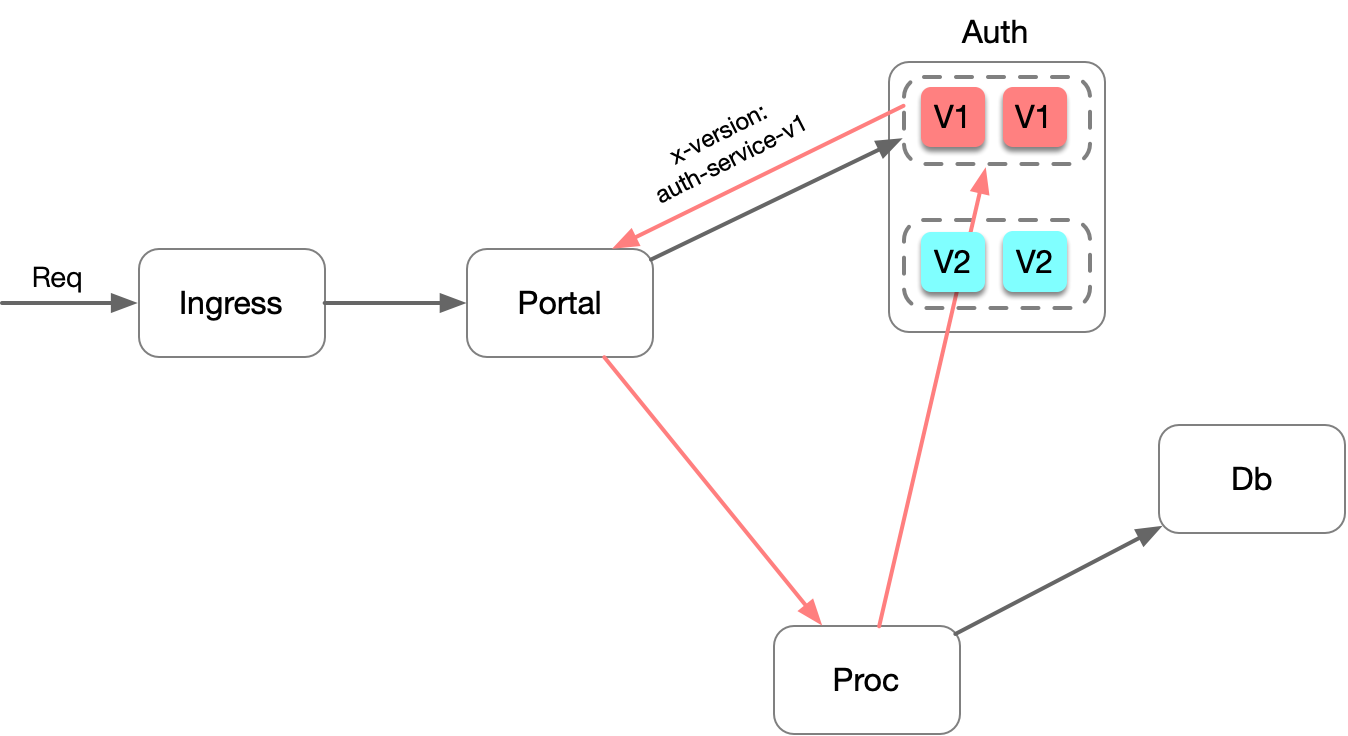
\includegraphics[height=5cm]{images/traffic_default_v1.png}
 \caption{流量默认发往v1}
 \label{fig:traffic_default_v1}
\end{figure}

\paragraph{路由规则更新}\label{section:update_route}
待前一步骤的配置完成,我们接着对路由规则进行配置修改:如图\ref{fig:vs_default_v2}所示,前两条规则并未发生修改,依然是优先根据头信息中的相关内容来进行流量的转发。关键在于将第三条规则的默认流量转发从v1改为v2。

\begin{lemma}
进行第三步的路由规则更新,将默认的流量转发目标从v1改为v2,不影响任何分布式事务的版本一致性,无论该分布式事务处于系统运行中的哪个阶段。
\end{lemma}

\begin{proof}
对于任何一个分布式事务T,若T在运行的过程中还未调用过auth-service,则请求的头信息中不包含相关的版本信息,依据规则T将使用v2版本,不违背版本一致性;若T在过往子事务的运行过程中调用过auth-service,则请求的头信息中必然包含相关的版本信息,此时路由规则将进行相关的头信息版本匹配,并转发往同一版本的auth-service,保证了版本一致性;若T在将来的运行过程中不会再调用auth-service,同样不违背版本一致性。因此证明了进行第三步\ref{section:update_route}的路由规则更新,任何分布式事务T都满足版本一致性的要求。
\end{proof}

\begin{figure}[ht]
 \centering
 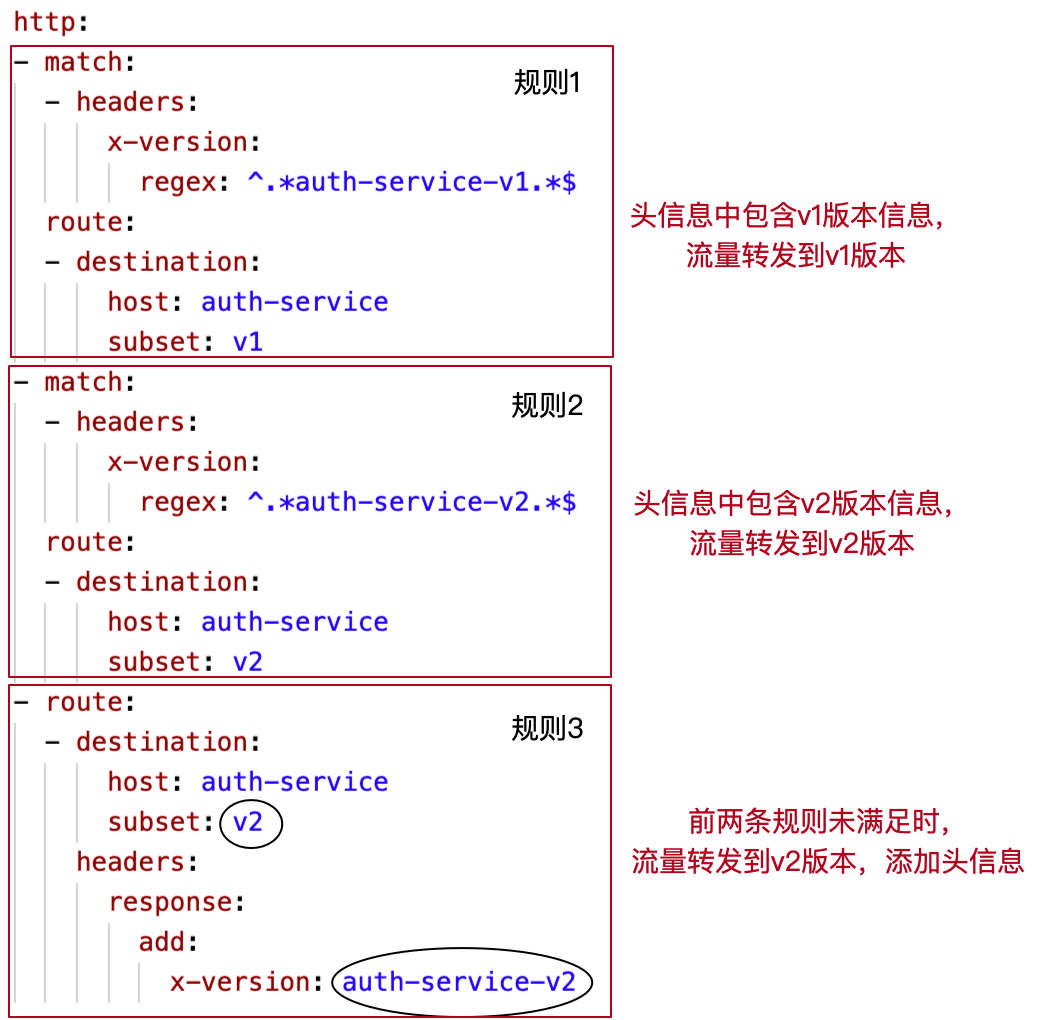
\includegraphics[height=8cm]{images/vs_default_v2.png}
 \caption{默认发往v2路由规则}
 \label{fig:vs_default_v2}
\end{figure}

更新完路由规则对应的系统运行状态如图\ref{fig:traffic_v1v2}所示,新产生的请求将发往新版本v2,运行中的请求则依据头信息内容进行匹配。
\begin{figure}[ht]
 \centering
 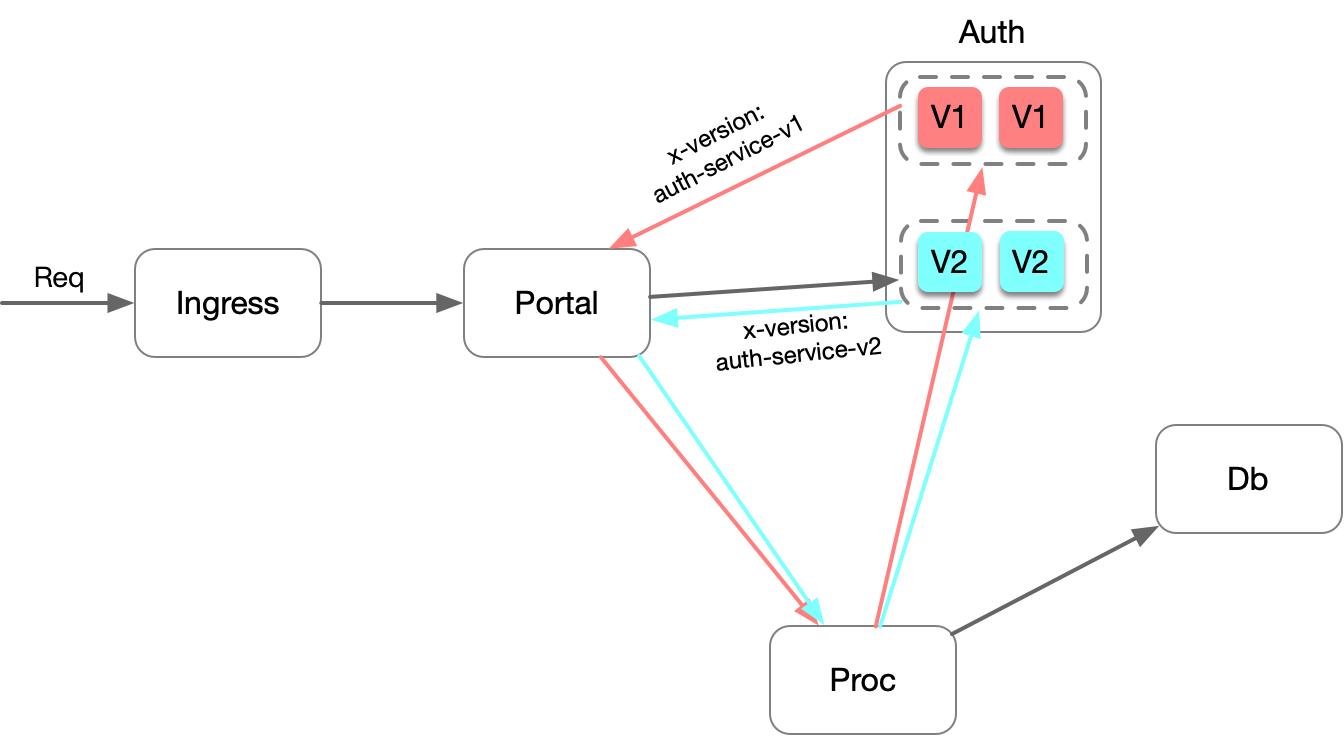
\includegraphics[height=5cm]{images/traffic_v1v2.png}
 \caption{新流量发往v2}
 \label{fig:traffic_v1v2}
\end{figure}

\paragraph{旧版本撤销请求}
完成前述步骤后,我们便完成了新旧版本流量的正确导向,新产生的用户请求也可以及时地使用新版本的服务。进一步我们希望能够及时地对旧版本的服务实例进行撤销,避免其长时间地占用系统的资源。我们需要进行判断:何时旧版本的服务实例上的事务全部结束且不会再为其它事务提供服务?这时,便需要使用TraceManager容器中所保存的TraceidSet。具体实现包括以下步骤:
\begin{enumerate}
	\item 阻塞访问旧版本:当收到旧版本的撤销请求时,阻塞所有调用旧版本服务实例的新请求,即头信息中不存在对应版本信息的流量,同时直接返回503(Service Not Available)错误,在调用方侧执行重试机制,此时调用方将应用较新的路由规则,流量被转发到新版本的服务中。从而保证了不会再有新请求调用到旧版本服务实例,并且对TraceManager容器中保存的TraceidSet执行加锁,不再向其中添加traceid,此时TraceidSet保存了所有调用过旧版本服务实例的分布式事务id。流程如图\ref{fig:block_and_retry}所示;
	\begin{figure}[ht]
	 \centering
	 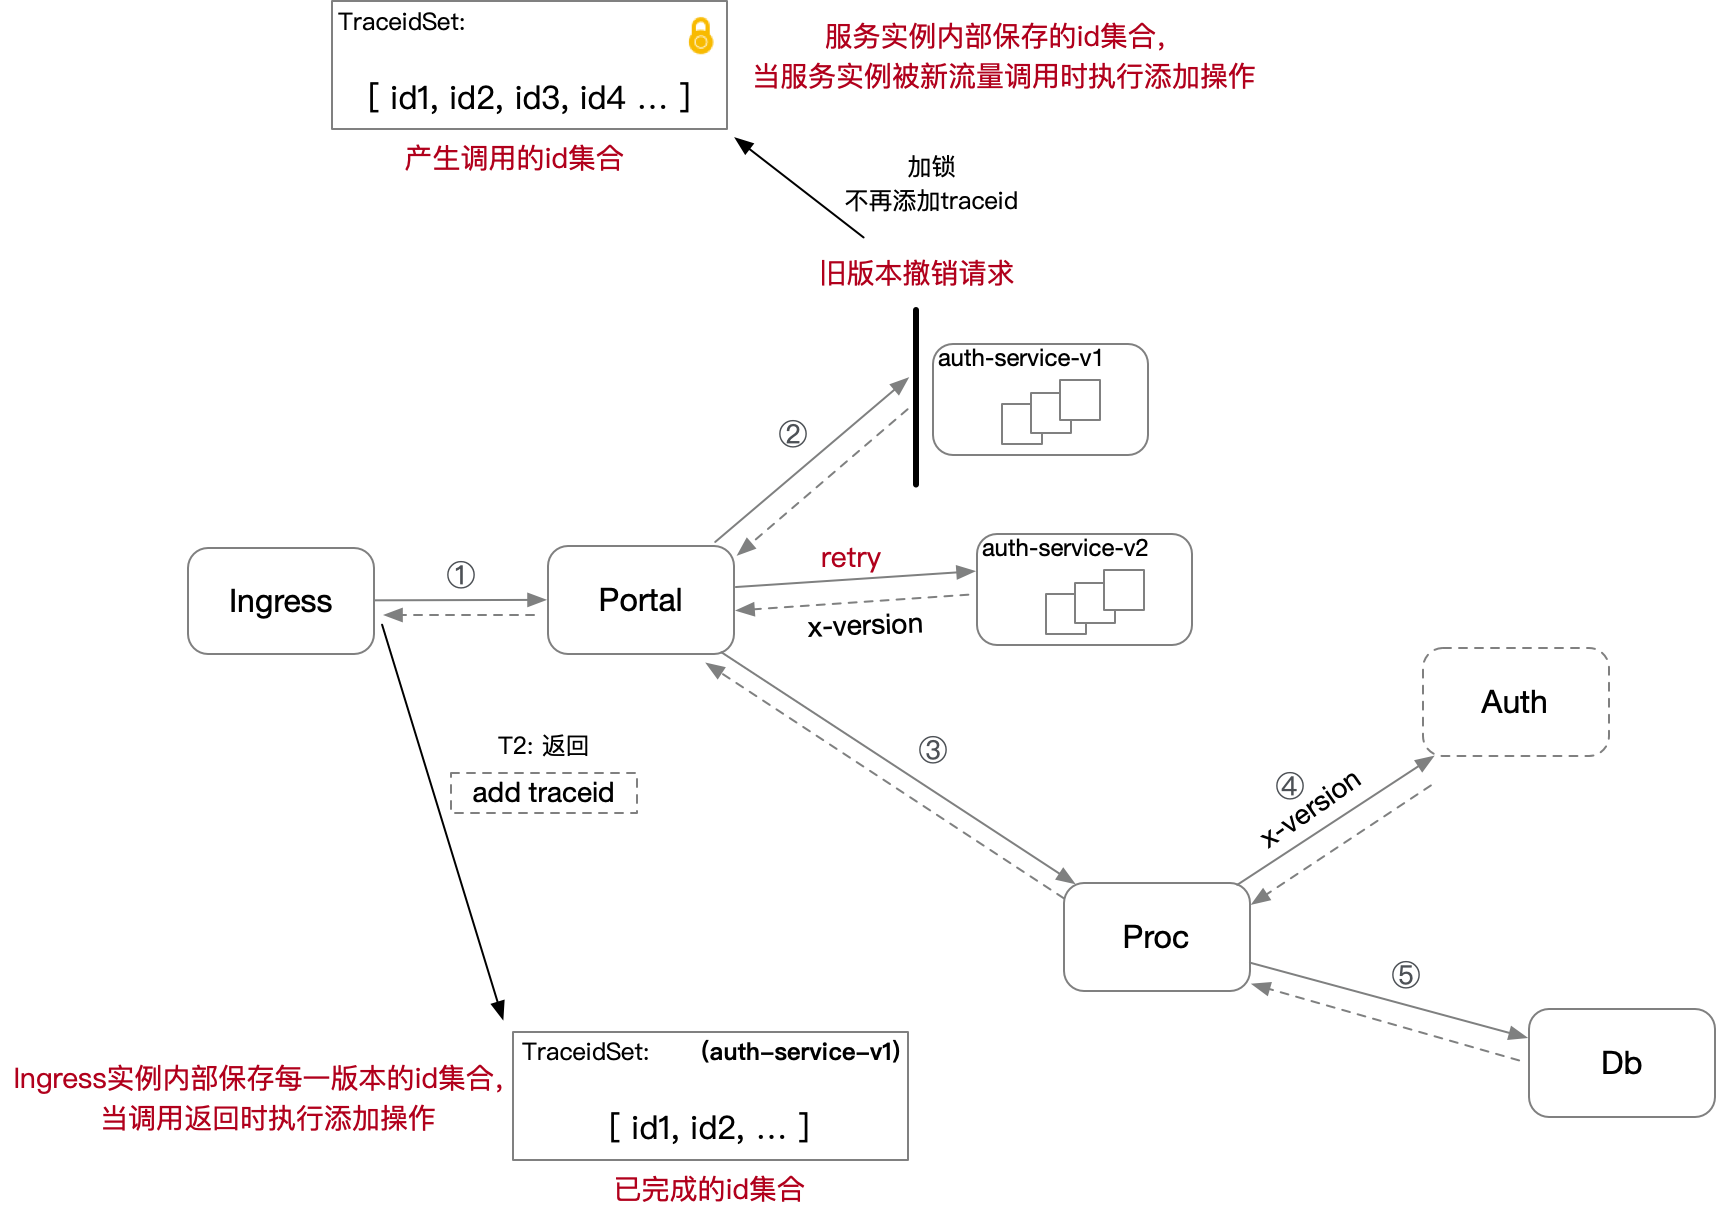
\includegraphics[height=10cm]{images/block_and_retry.png}
	 \caption{阻塞访问旧版本}
	 \label{fig:block_and_retry}
	\end{figure}

	\item 同步Traceid集合:将所有旧版本实例中所保存的TraceidSet发送至Ingress Gateway。Ingress Gateway此时暂时阻塞添加Traceid,将收到的TraceidSet和自己内部保存的TraceidSet进行同步,求得差集DiffSet。此差集便表示了所有调用过旧版本服务,但还未将运行结果返回给Ingress Gateway的分布式事务id集合。示例如图\ref{fig:sync_traceid}所示;
	\begin{figure}[ht]
	 \centering
	 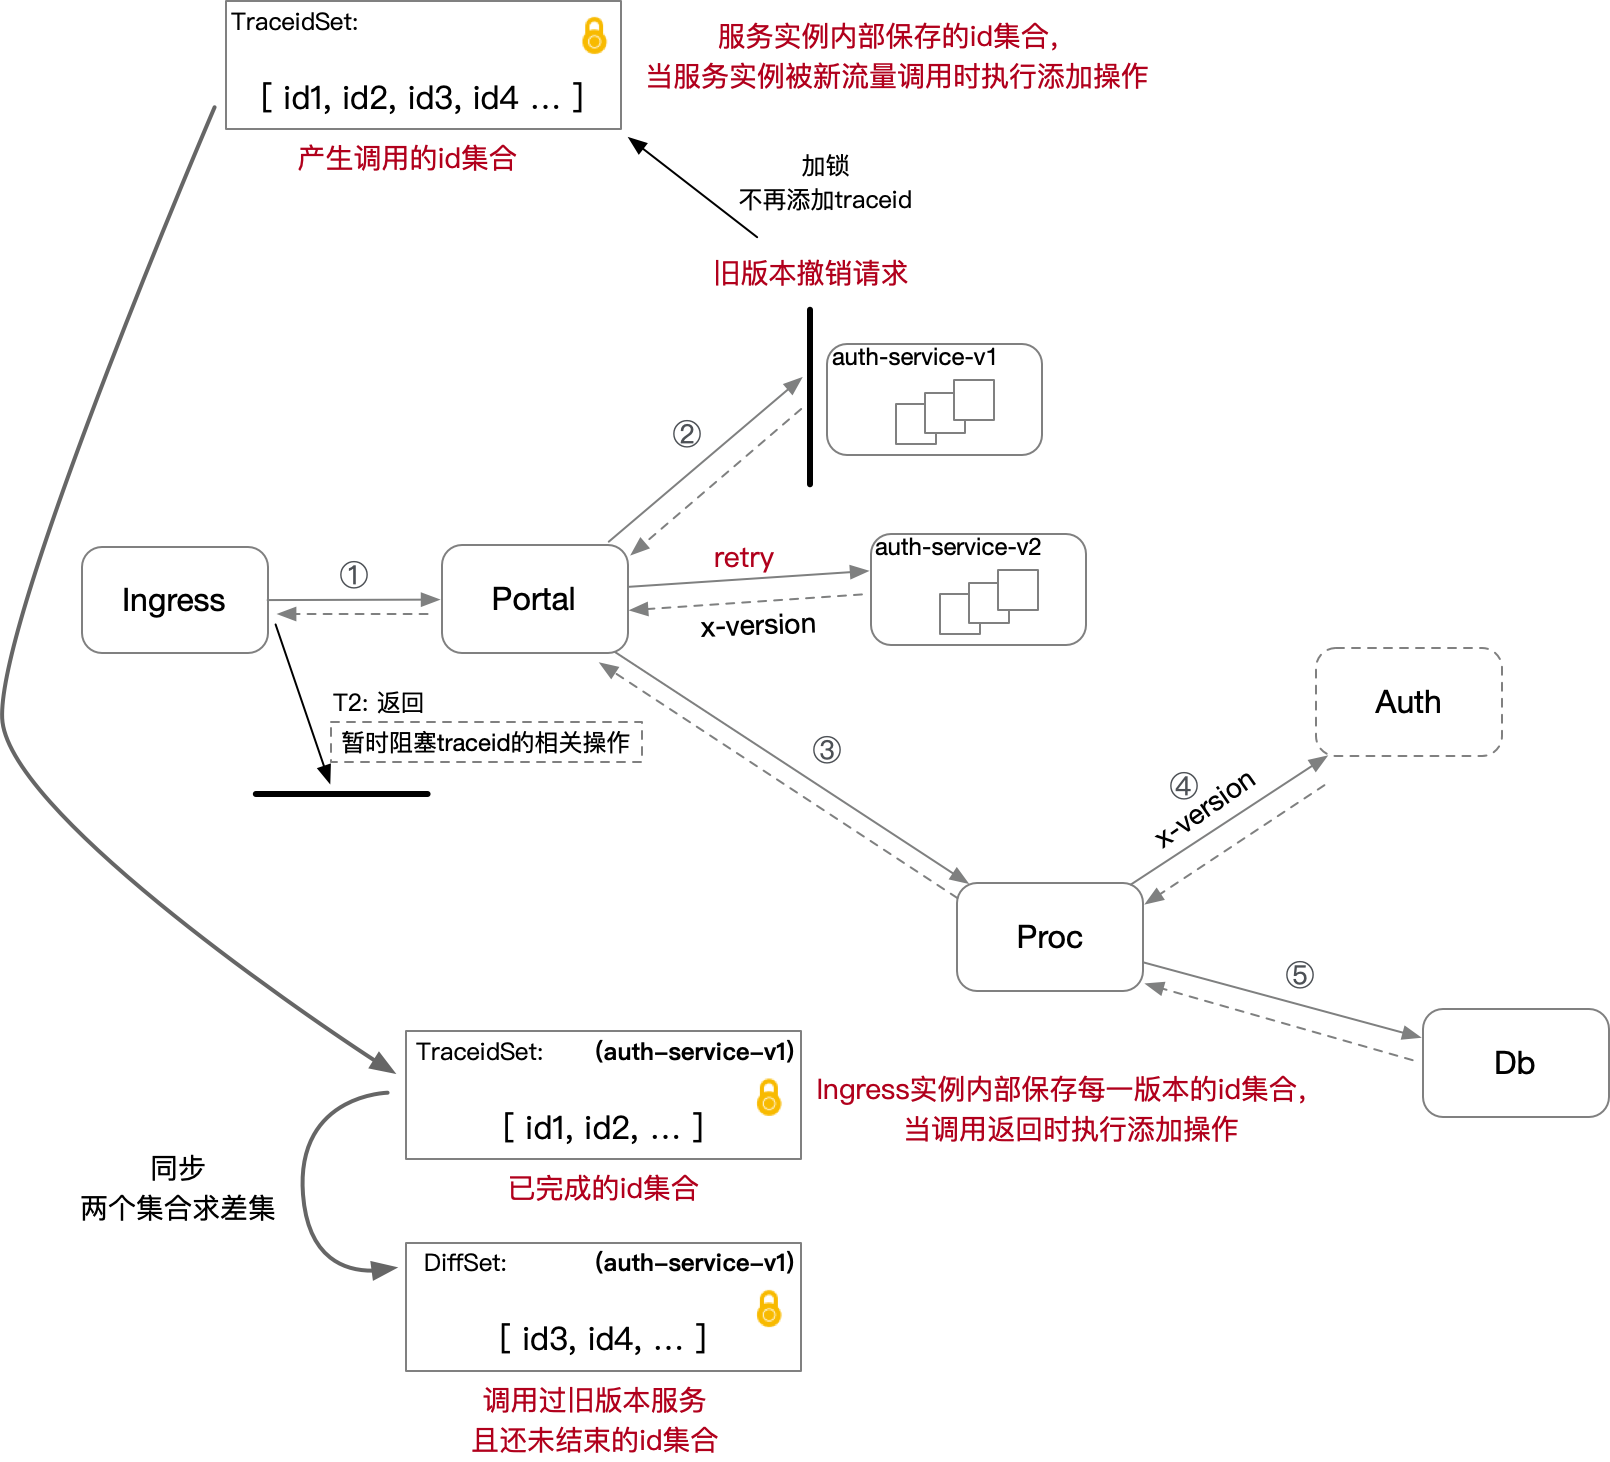
\includegraphics[height=10cm]{images/sync_traceid.png}
	 \caption{同步Traceid集合}
	 \label{fig:sync_traceid}
	\end{figure}

	\item 利用差集完成旧版本的撤销:在得到前一步骤的差集结果DiffSet后,不再阻塞Traceid的相关操作,对于收到的每一个Traceid,将其从DiffSet中删除,表示该分布式事务运行完成并返回结果。当差集DiffSet最终删除为空集时,我们便可以做出推断:所有已调用过旧版本服务的分布式事务均已返回结果,旧版本服务实例可被撤销。具体如图\ref{fig:wait_for_revoke}所示;
	\begin{figure}[htbp]
	 \centering
	 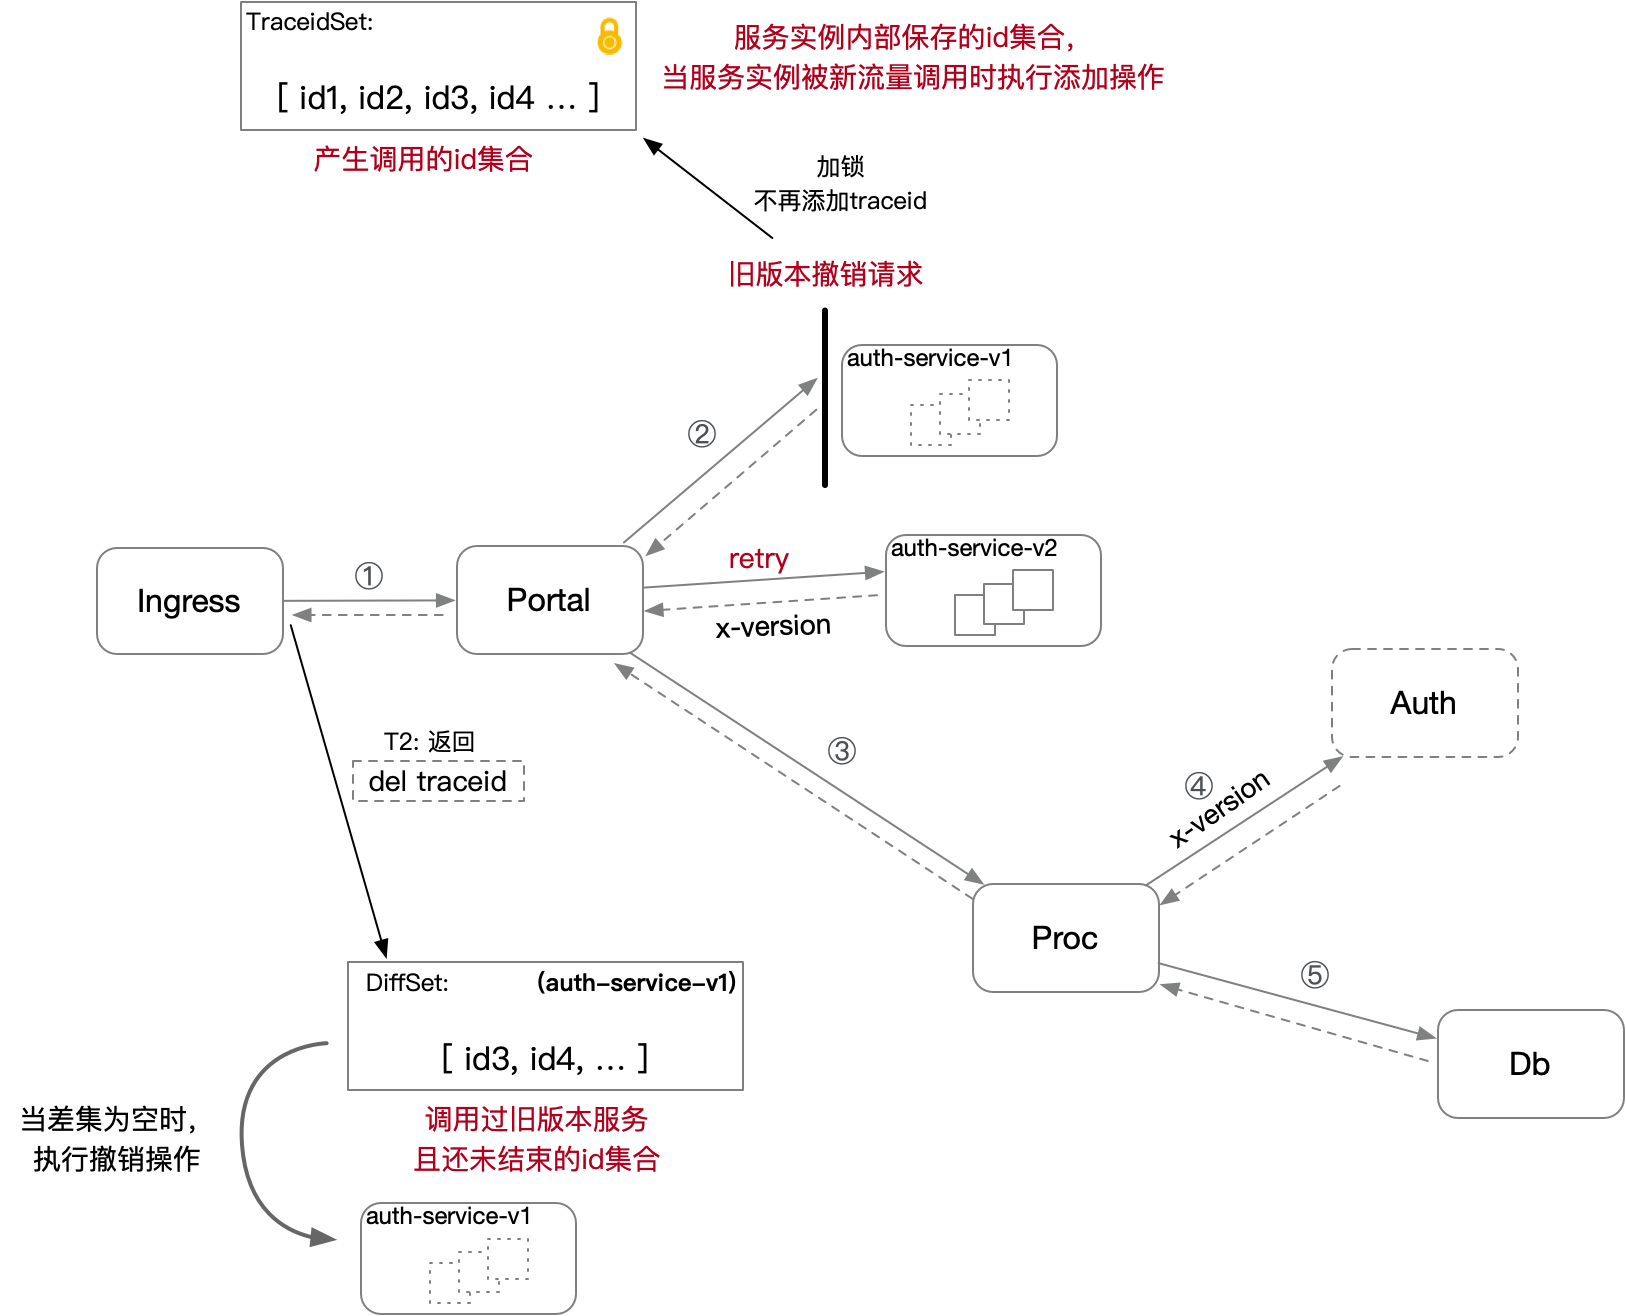
\includegraphics[height=10cm]{images/wait_for_revoke.png}
	 \caption{利用差集完成旧版本的撤销}
	 \label{fig:wait_for_revoke}
	\end{figure}
\end{enumerate}

\paragraph{旧版本撤销与清理操作}
完成前述步骤后,我们就可以安全地撤销掉旧版本的所有服务实例,同时对相关的配置进行清理,还原成类似步骤1\ref{section:setup}中的初始状态,只是相关的版本从v1变更为v2,为下一次更新操作奠定基础。具体的路由规则、版本规则和系统运行状态分布如图\ref{fig:vs_all_v2}、\ref{fig:dr_v2}、\ref{fig:traffic_all_v2}所示
\begin{figure}[h]
\centering
\begin{minipage}[t]{0.48\textwidth}
\centering
\centerline{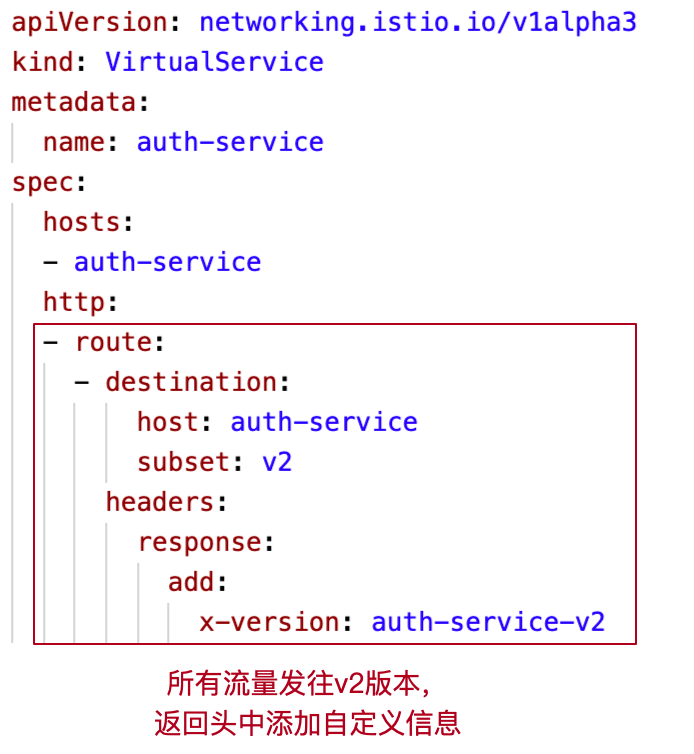
\includegraphics[width=7cm]{vs_all_v2.png}}
\caption{v2路由规则}
\label{fig:vs_all_v2}
\end{minipage}
\begin{minipage}[t]{0.48\textwidth}
\centering
\centerline{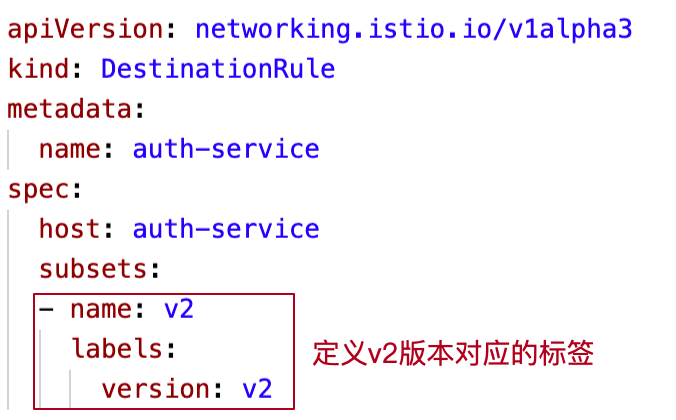
\includegraphics[width=6cm]{dr_v2.png}}
\caption{v2版本规则}
\label{fig:dr_v2}
\end{minipage}
\end{figure}
\begin{figure}[ht]
 \centering
 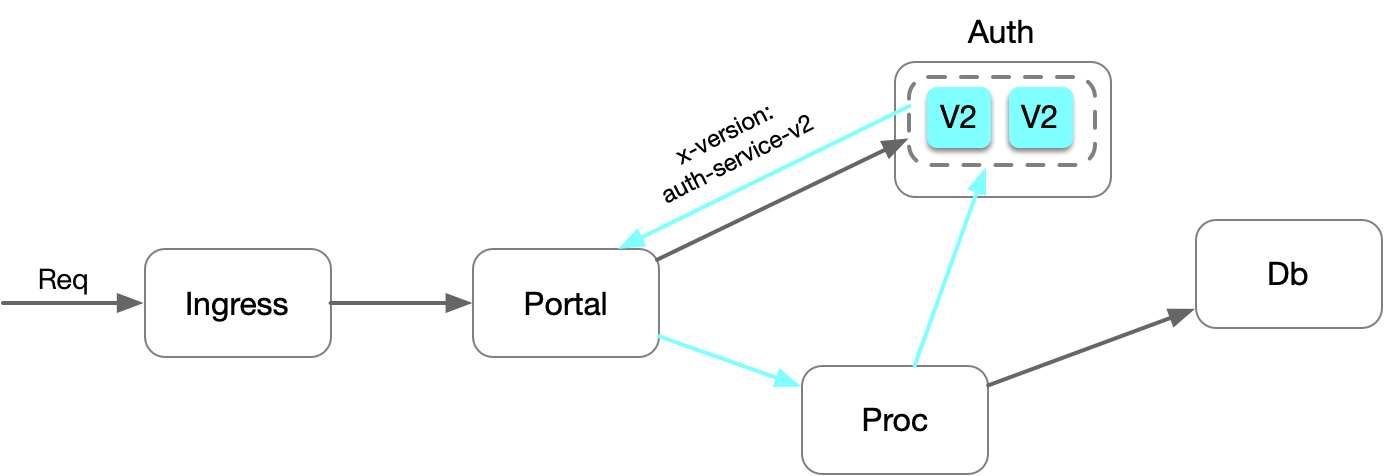
\includegraphics[height=5cm]{images/traffic_all_v2.png}
 \caption{流量全部发往v2}
 \label{fig:traffic_all_v2}
\end{figure}



\section{人机物融合平台架构与技术集成} 

互联网的快速发展催生新技术与新业务的出现。软件从单纯的信息处理环节逐步成为了应用价值观的主要载体,并形成将人、计算机以及物理世界相连接的人机物融合软件新形态。

而当前主流软件技术对人机物开放环境下资源的有效协同的支持存在较明显的不足。人机物融合平台旨在结合软件代理、软件协同等方面的技术创新,兼容地扩展已被广泛实践的主流技术,构建开放协同场景下针对性与实用性较好的技术框架,以灵活地协同管理各种自治的人机物资源,并支撑人机物融合应用系统的运行。

\subsection{总体的设计和结构}

相较于传统的计算资源管理平台,人机物融合平台除了需要能接入分布于云、网、端的各类人机物资源,还需要制定一套满足人机物资源开放性的资源协作规范,在统一协作规范的基础下,组合实现人机物融合应用的完整逻辑。

融合平台的运行环境基于当前最主流的容器化编排系统\textbf{Kubernetes},在其上制定了一套人机物资源的描述规范,设计了一种消息驱动的人机物资源协作模型,构建了一套面向人机物融合的资源服务治理框架。

\begin{figure}[ht]
 \centering
 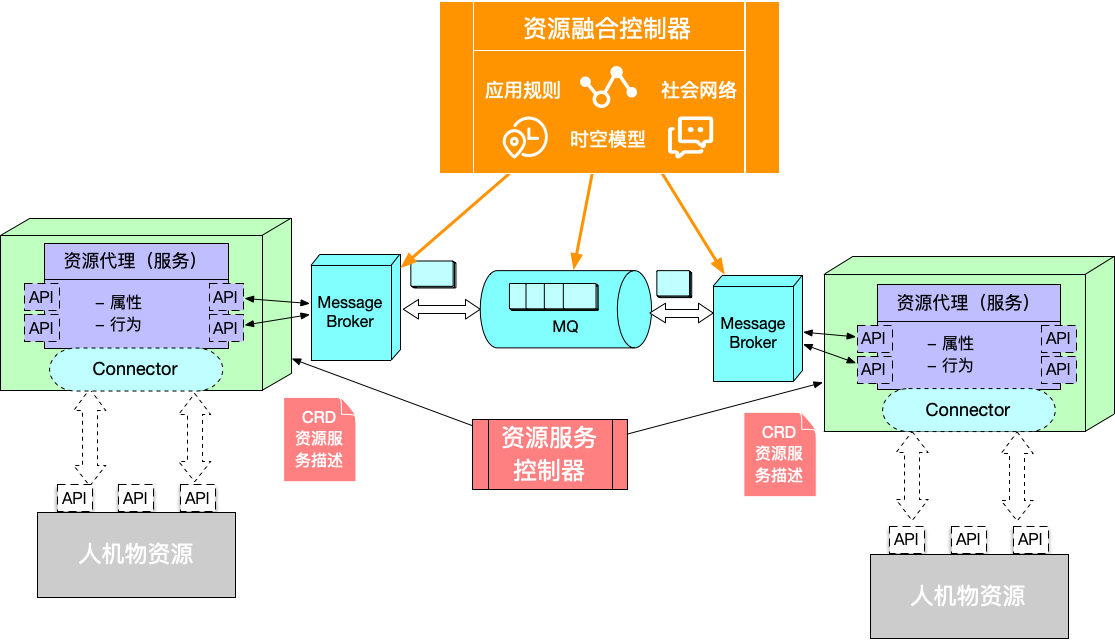
\includegraphics[height=8cm]{images/overview_arch.jpg}
 \caption{资源平台总体架构}
 \label{fig:singleblock}
\end{figure}

在融合平台中,人机物资源借助于微服务的形式,表示其在现实世界和信息世界中的状态及其具有的能力,称之为资源代理服务。资源代理服务间借助于专用的消息中间件进行通信,以消息驱动的方式进行松耦合的协作。为支持人机物融合应用的复杂使用场景,消息中间件在进行服务治理时,除了需要基于传统的服务质量等指标以外,还需要基于应用描述,综合考虑物理时空与社会关系等属性,生成自适应的消息路由规则。

从传统计算资源管理平台的角度来看,融合平台按照用户提供的人机物资源描述,维护资源代理服务和消息中间件等组件的运行状态;从人机物资源管理平台的角度来看,融合平台向下接入现实世界的各类人机物资源,向上层的资源代理服务与消息中间件,提供相对统一的资源访问接口。

\subsection{人机物资源的描述与编排}
实际的物理资源都要抽象成一种数据结构存储在系统中,系统同时要更新和维护它们。本软件平台通过\textbf{Kubernetes CRD}在系统中表示抽象资源,存储在\textbf{etcd}中,\textbf{Kubernetes Controller}负责维护它们,同步状态。
\subsubsection{人机物资源描述规范}
\textbf{CRD}是\textbf{CustomResourceDefinition}的简写,资源是\textbf{kubernetes}中的抽象概念,\textbf{CRD}是自定义的资源。

所有物理资源都要在系统中注册,且在系统中表达为\textbf{Resource CRD},需要使用一些参数描述资源。这些参数告诉了\textbf{Kubernetes}平台如何去访问资源并维护资源的状态。首先,资源需要一个唯一的标识。其次,因为需要使用探针去采集资源的各项信息,需要包含探针程序的镜像地址和启动命令以及启动参数。


\begin{table}[!htbp]
\centering
\begin{tabular}{ccc}
  \toprule
  字段& 类型& 意义\\
  \midrule
  ResourceKind& enum& 资源类型,包括人、机器、服务\\
  Icon& string& 标识位置,用于在前端显示\\
  Description& map[string]string& 资源描述\\
  AccessMode& ResourceAccessMode& 访问方式,独占或者共享\\
  AliasName& string& 资源别名\\
  ProbeSpec& ProbeSpec& 探针属性\\
  ConnectorSpec& ConnectorSpec& 连接器属性\\
  \bottomrule
\end{tabular}
\caption{ResourceSpec}
\end{table}

\begin{table}[!htbp]
\centering
\begin{tabular}{ccc}
  \toprule
  字段& 类型& 意义\\
  \midrule
  Enabled& bool& 决定是否启用探针\\
  Image& string& 探针的镜像\\
  Args& []string& 探针的启动参数\\
  Patchers& []FieldPatcher& 字段修改器\\
  \bottomrule
\end{tabular}
\caption{ProbeSpec}
\end{table}

\begin{table}[!htbp]
\centering
\begin{tabular}{ccc}
  \toprule
  字段& 类型& 意义\\
  \midrule
  Source& HTTPActionSpec& 操作接口\\
  Setters& []FieldSetter& 字段设置器\\
  \bottomrule
\end{tabular}
\caption{FieldPatcher}
\end{table}

\begin{table}[!htbp]
\centering
\begin{tabular}{ccc}
  \toprule
  字段& 类型& 意义\\
  \midrule
  Parser& string& 解析器\\
  Type& string& 类型\\
  Target& HTTPActionSpec& 操作接口\\
  \bottomrule
\end{tabular}
\caption{FieldSetter}
\end{table}

\begin{table}[!htbp]
\centering
\begin{tabular}{ccc}
  \toprule
  字段& 类型& 意义\\
  \midrule
  Action& string& 接口名称\\
  URL& string& 接口url\\
  Query& map[string]string& 对接口的查询参数\\
  Headers& map[string]string& 请求头\\
  \bottomrule
\end{tabular}
\caption{HTTPActionSpec}
\end{table}

\begin{table}[!htbp]
\centering
\begin{tabular}{ccc}
  \toprule
  字段& 类型& 意义\\
  \midrule
  Image& string& 连接器镜像\\
  Args& []string& 连接器的启动参数\\
  ListenPort& int32& 连接器监听的端口\\
  \bottomrule
\end{tabular}
\caption{ConnectorSpec}
\end{table}

\begin{table}[!htbp]
\centering
\begin{tabular}{ccc}
  \toprule
  字段& 类型& 意义\\
  \midrule
  Phase& enum& 状态(包括Pending、Running、Failed)\\
  ProbePhase& enum& 探针状态(包括NotReady、Pending、Synchronous和Failed)\\
  Bound& bool& 是否已经被绑定使用\\
  CreateTime& *metav1.Time& 创建时间\\
  StartTime& *metav1.Time& 各个组件都启动的时间\\
  \bottomrule
\end{tabular}
\caption{ResourceStatus}
\end{table}

\subsubsection{人机物资源的运行时编排}

\textbf{Linux}容器技术能够对应用及其整个运行时环境(包括全部所需文件)一起进行打包或隔离。从而让开发者可以在不同环境(如开发、测试和生产等环境)之间轻松迁移应用,同时还可保留应用的全部功能。

容器是虚拟化的主要形式之一,相比于虚拟机需要虚拟化基础硬件,每个虚拟机都运行一个操作系统,容器共享主机\textbf{OS},因此它们不需要启动\textbf{OS}或加载库。这使得容器更加高效和轻量。容器化应用程序可以在几秒钟内启动,与\textbf{VM}方案相比,应用程序的更多实例可以适应计算机。共享\textbf{OS}方法具有额外的好处,即减少维护(如修补和更新)开销。

\textbf{Kubernetes}提供了生产级容器编排服务,它是一种可自动实施 \textbf{Linux} 容器操作的开源平台。它可以帮助用户省去应用容器化过程的许多手动部署和扩展操作。\textbf{Kubernetes} 可为用户提供一个便捷有效的平台,让用户可以在物理机或虚拟机集群上调用和运行容器。\textbf{Kubernetes} 架构将集群分为不同的组件,这些组件要协同工作来维护集群的预期状态。

\textbf{Kubernetes Operator} 是一种封装、部署和管理 \textbf{Kubernetes} 应用的方法。\textbf{Operator} 是使用自定义资源(\textbf{CR})管理应用及其组件的自定义 \textbf{Kubernetes} 控制器。高级配置和设置由用户在 \textbf{CR} 中提供。\textbf{Kubernetes Operator} 基于嵌入在 \textbf{Operator} 逻辑中的最佳实践将高级指令转换为低级操作。自定义资源是 \textbf{Kubernetes} 中的 \textbf{API} 扩展机制。自定义资源定义(\textbf{CRD})会明确 \textbf{CR} 并列出 \textbf{Operator} 用户可用的所有配置。 \textbf{Kubernetes Operator} 监视 \textbf{CR} 类型并采取特定于应用的操作,确保当前状态与该资源的理想状态相符。

我们使用\textbf{Operator}的形式在\textbf{Kubernetes}中部署人机物融合平台。
\textbf{Resource CRD}由\textbf{Resource Controller}管理,控制器监控资源的状态,当监测资源的增删改事件时就会生成一个包含相关资源名称的\textbf{request}塞入工作队列,\textbf{Reconcile}方法每隔很短的一段时间被调用一次,从工作队列中取出一个\textbf{request}作为参数进行处理。

\textbf{Reconcile}首先根据\textbf{request}中包裹的资源名称和命名空间找到\textbf{Resource}的实例,如果是删除事件什么都不需要做,增改事件则会判断是否需要新建、更新、删除包含探针和连接器的\textbf{Deployment}资源以及\textbf{Service}资源。

控制器的实际工作就是把\textbf{Resource CRD}翻译成\textbf{Kubernetes}中的原生资源,\textbf{Deployment}会负责生产实际的\textbf{Pod}来运行\textbf{Probe}和\textbf{Connector}容器,\textbf{Service}用于暴露\textbf{Connector},让其他的应用可以访问它。

\subsection{消息驱动的人机物资源协作模型}

\subsubsection{资源接入层}

人机物融合场景下,为适配各类资源(特别是智能设备)连接方式的多样性,提高资源代理服务的可移植性以及通用性,平台提供了统一的资源接入层,资源代理服务通过资源接入层,以相对统一的资源访问接口与人机物资源进行交互。

资源接入层包含访问控制、状态缓存、访问请求映射等功能。资源接入层提供访问控制的功能,以保护敏感资源的访问;资源代理服务可向资源接入层描述自己所关心的资源状态,资源接入层会主动检查资源的状态是否发生变化(取决于资源实际接入平台的访问模式,也支持异步地订阅状态变化通知),如发生变化则通知资源代理服务更新数字对象状态。

对于资源接入层的访问请求映射功能。以智能设备为例,可借助于\textbf{Home Assistant}、\textbf{OpenHab}这类\textbf{IoT}管理平台进行接入,以提供资源的状态查询与操作接口,融合平台只需将统一的资源访问请求映射为\textbf{IoT}管理平台对应的请求即可。

除此之外,对于典型的边缘计算等三层网络访问受限的场景,资源代理服务无法直接访问到资源暴露出的操作接口。此时,资源接入层在资源代理服务所处的容器,与智能设备实际接入进程所处容器之间,建立点对点的隧道连接,以突破扁平容器网络模型的限制。

\begin{figure}[ht]
 \centering
 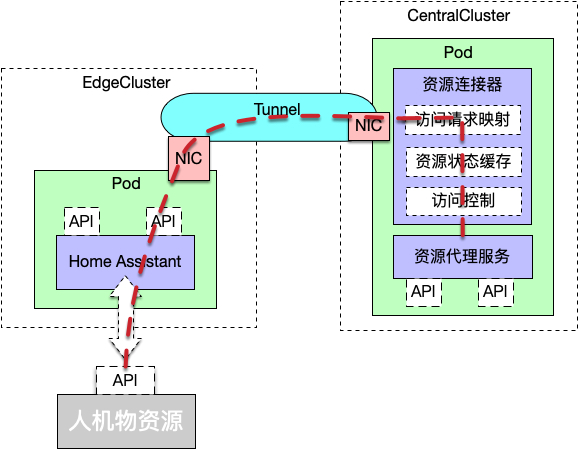
\includegraphics[height=8cm]{images/connector.jpg}
 \caption{资源接入层}
 \label{fig:singleblock}
\end{figure}

\subsubsection{资源代理服务}

资源代理服务除了需要提供其状态的描述信息之外,还需提供对应的操作接口,实际上以\textbf{RESTful API}的形式描述。目前我们采用传统的\textbf{MVC}架构,在\textbf{Spring Boot}框架上构建我们的资源代理服务。

资源代理主要分为两类: 智能设备和人。具体实现方面,资源代理服务在我们的平台上是一个一个的\textbf{Spring Boot}微服务,下面分别描述智能设备和人的资源代理服务的实现方式。

\begin{itemize}
	\item{\textbf{智能设备}}\\
	智能设备的资源代理相对固定,因为智能设备的功能是相对固定的,所以当资源代理部署完成之后,不需要对它的属性和功能接口进行大的修改。以空气净化器为例,在实现资源代理服务时,一方面开发人员对空气净化器进行建模,将空气净化器的属性信息和时空属性加入元模型,并按照资源接入层的规范提供相应的修改查询接口,另一方面开发人员需要封装资源接入层提供的资源互操作接口,生成对应的\textbf{RESTful API},使得用户可以通资源代理服务的接口来操控空气净化器。
\begin{scala}
    @PostMapping("/turnon")
    @Accessible("true")
    public String turnOnAirPurifier(){
        RestTemplate restTemplate = new RestTemplate();
        String url = "http://xxx/api/services/fan/turn_on";
        HttpEntity<String> request = new HttpEntity<>(
            new JSONObject().put("entity_id", "fan.xiaomi").toString(), 
            new HttpHeaders().setContentType(MediaType.APPLICATION_JSON)
        );
        return restTemplate.postForObject(url, request, String.class);
    }
\end{scala}
    \item{\textbf{人}}\\
    和智能设备相比,人的资源代理服务实现方面有一些区别,人的资源代理服务描述了在某个具体场景下该人所具有的能力,所以随着人的活动,他的资源代理服务会不断更新。举例来说,当人进入一个只有空气净化器的房间时,现实世界中的人就增加了一个使用空气净化器的能力,在这个场景下,人的资源代理服务就会增加操控空气净化器的接口。当这个人从房间离开,进入一个有咖啡机的房间,那么现实世界中的人会失去使用空气净化器的能力,增加使用咖啡机的能力,相应地,人的资源代理服务也会相应更新,删除操控空气净化器的接口,增加操控咖啡机的接口。
\end{itemize}

\subsubsection{消息中间件}
%\ref{fig:singleblock}
\begin{figure}[ht]
 \centering
 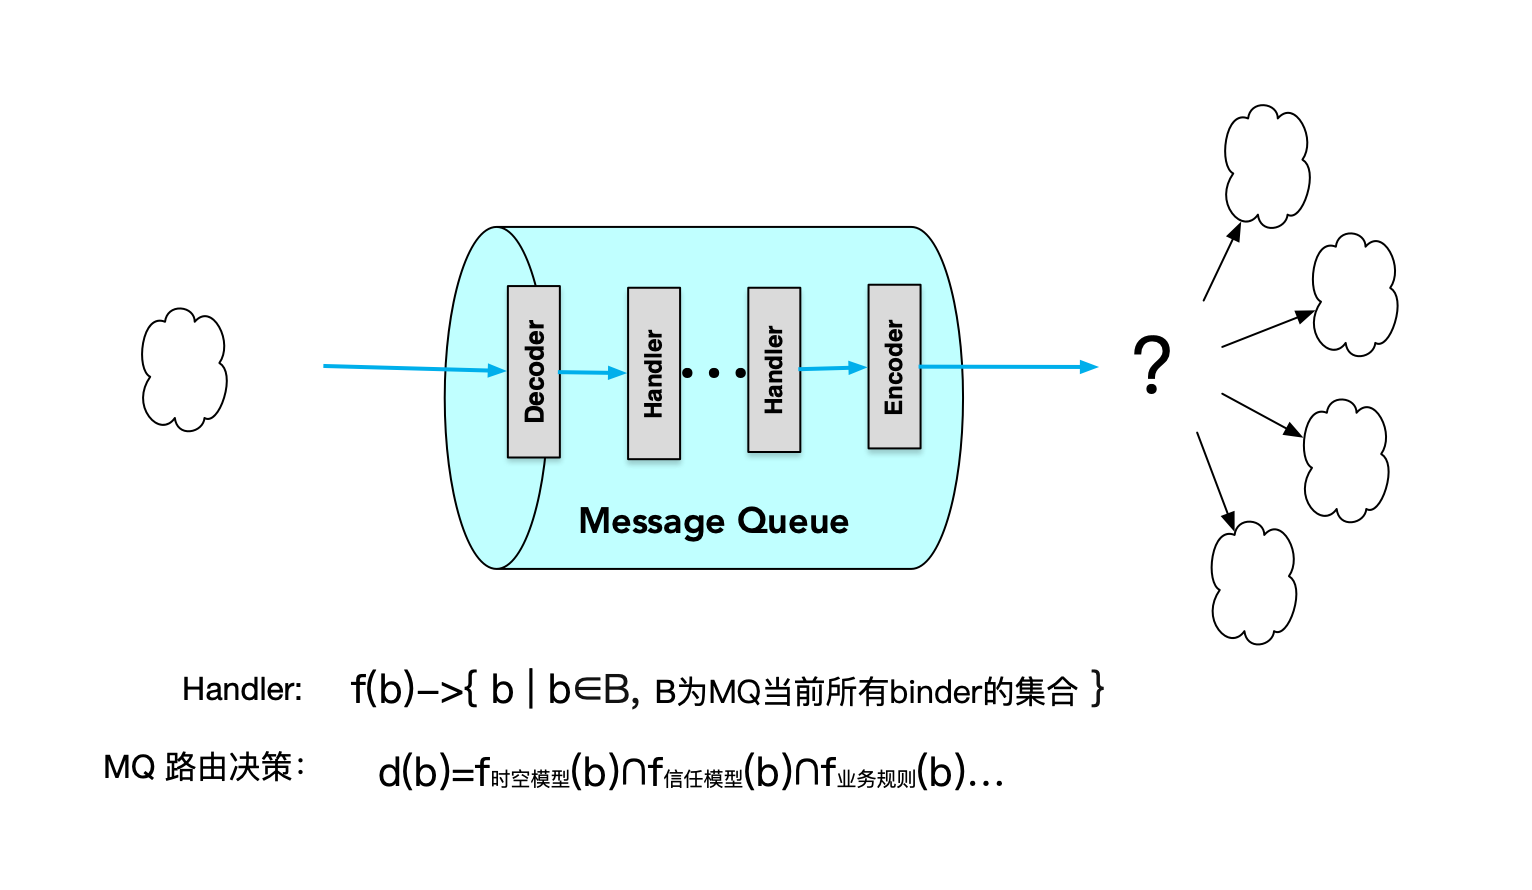
\includegraphics[height=5cm]{images/mq_architecture.jpg}
 \caption{mq架构图}
 \label{fig:singleblock}
\end{figure}
通过分析“人机物融合的云计算平台”的实际应用场景,首先我们需要一个松耦合的,消息驱动的服务治理平台来对资源代理服务进行治理,这样才能更好地描述和匹配现实世界中实际的业务场景需要。同时我们考虑将时间空间等现实世界中影响场景实际走向的因素作为通信协议的一部分,通过制定消息路由策略来反应现实世界中的时空属性对服务治理的影响,所以综合以上两点,我们基于Netty实现了一个简单的消息中间件来支撑平台的消息通信模块。

\begin{itemize}
    \item {\textbf{基于Java语言编写,网络通讯依赖Netty}}\\
    平台中的消息中间件是基于Netty实现的,Netty是一个异步的,事件驱动的,可以用来快速开发可维护的高性能的服务器和客户端的网络应用框架,它极大地简化了网络编程,允许用户从TCP/UDP层自定义通信协议。目前比较流行的消息队列,例如RabbitMQ,ActiveMQ等都利用Netty来支撑项目中的消息通信模块。
    \item {\textbf{通过定义topic来区分不同类型的资源代理服务}}\\
    当服务绑定到messageBroker上时,需要声明自己的topic,例如不同品牌的咖啡机的topic都是coffeeMachine,这样可以对同种类型的资源聚合,对不同类型的资源进行区分。
    \item {\textbf{采用Kryo进行消息的网络序列化传输}}
    \item{\textbf{支持基于时空属性的消息路由策略}}\\
    基于IndoorGML建模规范对静态空间进行建模,维护空间中不同资源实体之间的距离信息,根据距离信息构建路由表,定期将最新的路由表发送给消息中间件。
\end{itemize}
\newpage
\paragraph{消息模型}
平台中的消息模型由请求消息和接收消息两种类型,分别由图2和图3表示。
\begin{figure}[ht]
 \centering
 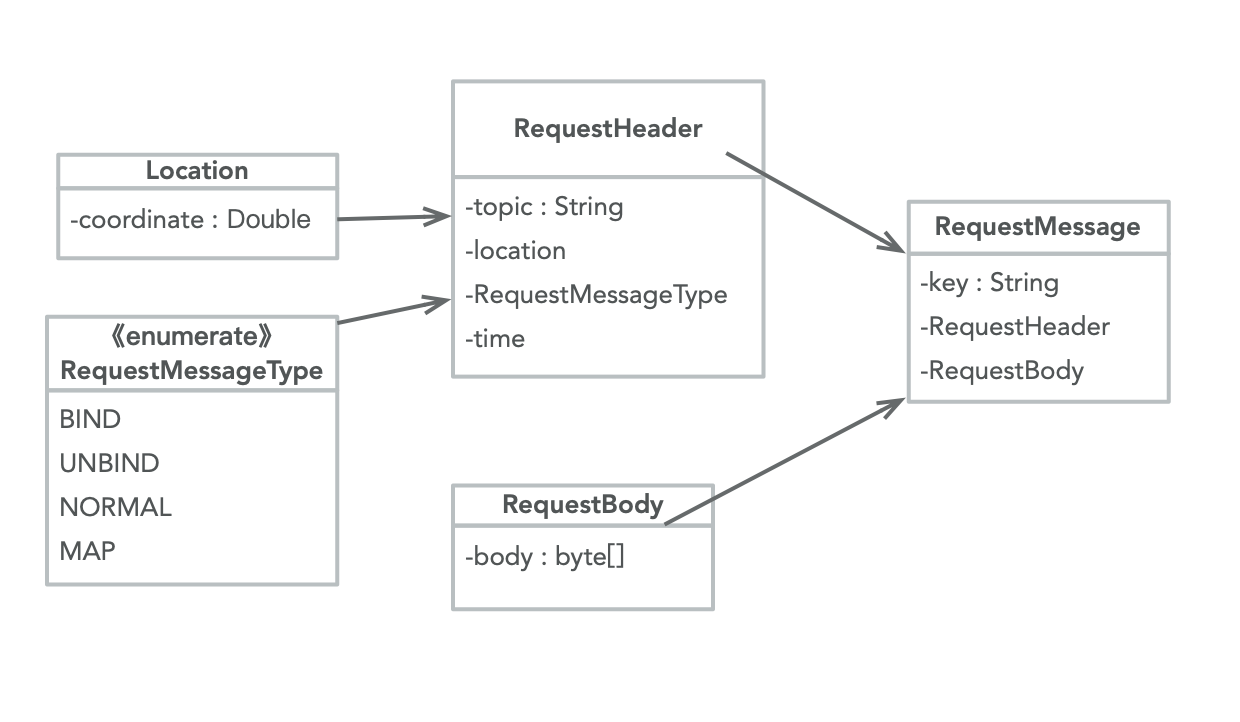
\includegraphics[height=5cm]{images/request_msg.png}
 \caption{请求消息模型}
 \label{fig:singleblock}
\end{figure}
\begin{figure}[ht]
 \centering
 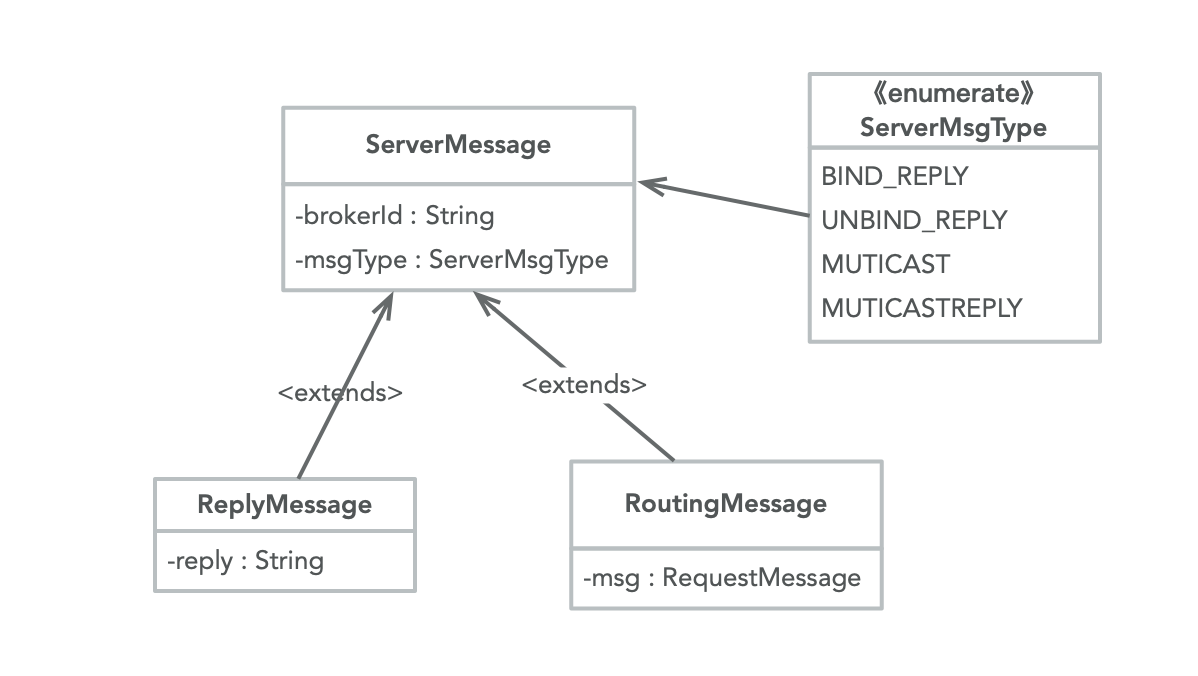
\includegraphics[height=5cm]{images/server_msg.png}
 \caption{接收消息模型}
 \label{fig:singleblock}
\end{figure}
\paragraph{消息序列化}
我们基于kryo来实现消息的序列化,主要利用KryoCodecUtil和KryoSerialize来完成消息的序列化和反序列化工作。
\begin{scala}
 public class KryoSerialize {
    private KryoPool pool;
    private Closer closer = Closer.create();
    public KryoSerialize(final KryoPool pool) {
        this.pool = pool;
    }

    public void serialize(OutputStream output, Object object) throws IOException {
        try {
            Kryo kryo = pool.borrow();
            Output out = new Output(output);
            closer.register(out);
            closer.register(output);
            kryo.writeClassAndObject(out, object);
            pool.release(kryo);
        } finally {
            closer.close();
        }
    }
    public Object deserialize(InputStream input) throws IOException {
        try {
            Kryo kryo = pool.borrow();
            Input in = new Input(input);
            closer.register(in);
            closer.register(input);
            Object result = kryo.readClassAndObject(in);
            pool.release(kryo);
            return result;
        } finally {
            closer.close();
        }
    }
}
\end{scala}
将kryo作为成员变量加入Netty的ByteToMessageDecoder和MessageToByteEncoder中,利用上面我们实现的kryo序列化和反序列化方法实现Netty中消息的编码和解码。
\begin{scala}
 public class RequestDecoder extends ByteToMessageDecoder {
    final public static int MESSAGE_LENGTH = MessageCodecUtil.MESSAGE_LENGTH;
  
    private MessageCodecUtil util; //kryo
    public RequestDecoder(MessageCodecUtil messageCodecUtil) {
        this.util = messageCodecUtil;
    }
    @Override
    protected void decode(ChannelHandlerContext ctx,
                          ByteBuf in, List<Object> out) throws Exception {
      	......
        Object obj = util.decode(messageBody);
      	......
     }
}
\end{scala}

\begin{scala}
 public class ResponseDataEncoder extends MessageToByteEncoder<Object> {
    private MessageCodecUtil util;
    ResponseDataEncoder(MessageCodecUtil messageCodecUtil) {
        this.util = messageCodecUtil;
    }
    @Override
    protected void encode(ChannelHandlerContext ctx, Object msg
                          , ByteBuf out) throws Exception {
        util.encode(out, msg);
    }
}
\end{scala}

\paragraph{MessageBroker实现}
\begin{itemize}
    \item {\textbf{客户端管理}}\\
    我们定义一个ClientInfo对象来描述注册在消息中间件上的客户端信息。
    
    \begin{figure}[ht]
    \centering
    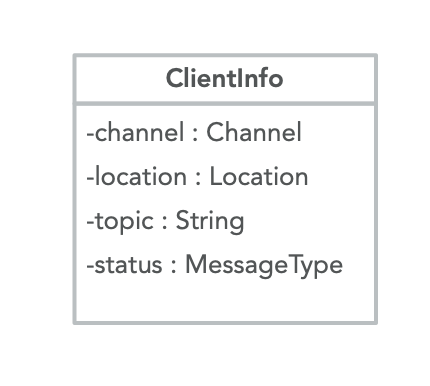
\includegraphics[height=5cm]{images/channelInfo.jpg}
    \caption{ClientInfo类图}
    \label{fig:singleblock}
    \end{figure}
    
    channel表示客户端通信的通道信息,location记录该client对应的资源代理服务的位置信息,topic代表该client对应的资源代理服务的类型,status表示该client目前的连接状态。
    
    我们用ConcurrentHashMap在内存中存放所有的ClientInfo。当有client发送bind请求时,messagebroker会先遍历ConcurrentHashMap,然后将新的client加入map中;相应地,当有client发送unbind请求时,messagebroker会先遍历ConcurrentHashMap,然后将对应的client状态改为DEAD;当客户端发送常规消息时,会查看location信息,保持location最新。
    \item {\textbf{消息路由}}\\
    当服务绑定到messageBroker上时,需要声明自己的topic,例如不同品牌的咖啡机的topic都是coffeeMachine,这样可以对同种类型的资源聚合,对不同类型的资源进行区分。
\end{itemize}

\paragraph{Producer/Consumer实现}
消息队列中的Producer发送消息,Consumer接收消息并对消息处理。其实在大部分情况下,Producer也需要接收消息,Consumer也需要发送消息,所以我们这里对他们一并看待,统称为Client,我们的Client也是基于Netty实现的,区别是在启动时,我们只给Client的workGroup分配了一个线程,所以可以理解为Client只能通过唯一的channel发送消息。我们给Client封装了ClientMessageSender来发送消息,ClientMessageHandler来接收消息。
\begin{itemize}
    \item {\textbf{绑定/解绑}}\\
\begin{scala}
    public synchronized void bind(String key,RequestHeader requestHeader
                          ,RequestBody requestBody){
           ……
           channelFuture.channel().writeAndFlush(bindMessage);
           notify();
    }

    public synchronized void unbind(String key,RequestHeader requestHeader
                            ,RequestBody requestBody){
           ……
           channelFuture.channel().writeAndFlush(unbindMessage);
           try {
                channelFuture.channel().closeFuture().sync();
           } catch (InterruptedException e) {
                e.printStackTrace();
           }
    }
\end{scala}
    \item {\textbf{发送业务消息}}\\
\begin{scala}
    public void sendMessage(RequestHeader requestHeader,RequestBody requestBody){
        try {
           wait();
        } catch (InterruptedException e) {
           e.printStackTrace();
        }
        ……
        channelFuture.channel().writeAndFlush(requestMessage);
    }
\end{scala}
    \item {\textbf{接收消息}}\\
\begin{scala}
  /**
   * 继承ServerMessageHandler类,用来接收mq发送来的消息
   * 其中有一个channel变量,调用channel.writeAndFlush()方法可以向mq发送答复消息
   * responseMessage()对应于sendMessage()方法
   * ackMessage()对应于bind()和unbind()方法
   */
   public class ResponseMessageReceiver extends ServerMessageHandler {
    @Override
    public void responseMessage(RequestMessage requestMessage) throws InterruptedException {
       ……
    }

    @Override
    public void ackMessage(String msg) {
        ……
    }
}
\end{scala}
\end{itemize}

\subsection{面向人机物融合的资源服务治理框架}
\subsubsection{资源服务发现}
资源服务是只有资源属性和资源能力的微服务,对外提供Restful API,我们的平台会为每一个资源服务生成一个消息适配器来支持资源服务发现,消息适配器的作用是自动地为资源服务添加基于消息中间件的消息通信模块,使得资源代理中的Restful API中的业务规则能在平台中以消息的形式在资源服务之间传递。总结来说,在保留资源代理本身的业务逻辑的同时,支撑平台的资源服务发现。
\begin{figure}[ht]
 \centering
 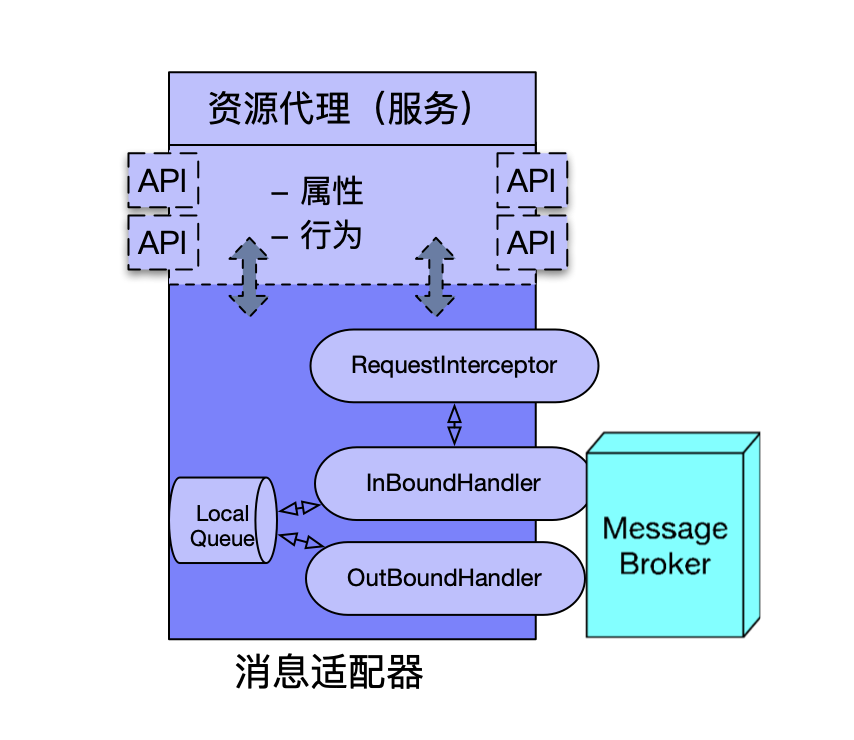
\includegraphics[height=5cm]{images/msg_adapter.png}
 \caption{消息适配器架构图}
 \label{fig:singleblock}
\end{figure}

 \begin{figure}[ht]
 \centering
 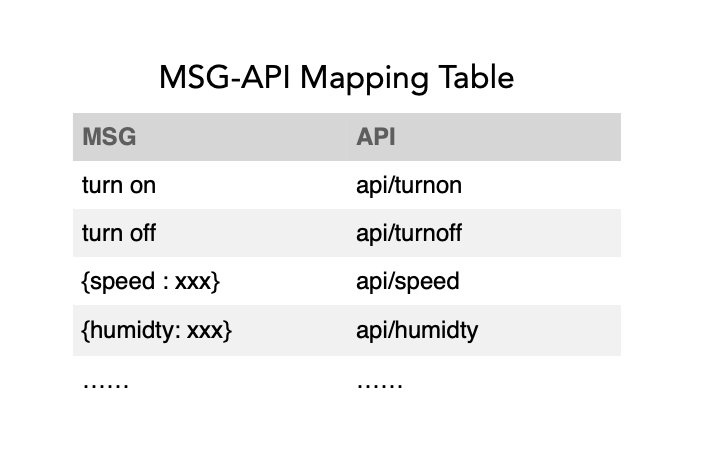
\includegraphics[height=5cm]{images/msg-api_mapping_table.png}
 \caption{“消息-接口”映射表}
 \label{fig:singleblock}
\end{figure}

\begin{itemize}
    \item {\textbf{整体架构}}\\
    消息适配器主要由InBoundHandler,OutBoundHandler,LocalQueue三部分组成,InBoundHandler会将从消息中间件中接收到的业务消息存入LocalQueue中,OutBoundHandler会监听LocalQueue,如果LocalQueue非空,就会根据用户事先定义的"消息-接口映射表",调用对应的Restful API或消息进行处理,并将处理完成的Ack发送给消息中间件。对于人的资源服务则需要单独考虑,人的资源代理往往作为整个消息流程的发起者,除了InBoundHandler,OutBoundHandler,LocalQueue三部分之外,人的资源代理服务的消息适配器需要为人动态生成Restful API来发起整个消息流程。换言之,人的资源代理的Restful API的作用是发起某个消息流程。 
    \item {\textbf{InBoundHandler实现}}\\
    InBoundHandler的实现比较简单,直接继承mq
    client的ServerMessageHandler类,重写ServerMessageHandler的responseMessage方法,该方法会接收到mq发送过来的消息,将接收到的消息存入Local Queue中,并回复mq消息已经收到。
    \begin{scala}
   @Override
    public void responseMessage(RequestMessage requestMessage) throws InterruptedException {
        try {
            String s = requestMessage.getRequestBody().getBody();
            messageQueue.add(s);
            this.notify();
            ......
            this.channel.writeAndFlush(reply);
            ...
        } catch (UnsupportedEncodingException e) {
            e.printStackTrace();
        }
    }
\end{scala}

    \item {\textbf{OutBoundHandler实现}}\\
    OutBoundHandler用于发送消息,OutBoundHandler的成员变量中需要一个资源代理的RestController实例,此外还需要消息和接口之间的映射表(图8)。这样当Local Queue非空时,每次获取一个请求信息,可以找到对应的消息内容,将消息通过发送给Consumer,当获取到的是消息时,通过找到对应的请求信息,调用RestController实例中的对应的接口执行相应的业务代码。
    
    \item{\textbf{人的资源代理Restful API实现}}\\
    对于现实世界中人可以使用的智能设备,在平台中,这些资源的资源代理会向消息中间件发送心跳消息来表示它们的占用情况,当人的资源代理启动之后,当接收到这些资源代理发送的广播消息,资源代理适配器会为人生成对应的Restful API来表示人目前具有的能力,这些接口中的代码逻辑比较简单,主要是生成调用不同资源代理的消息,并将消息加入LocalQueue中,这样当这些Restful API被请求时,OutBoundHandler就会发出LocalQueue中的消息,整个消息流程启动。
\end{itemize}
\subsubsection{资源服务路由}
资源服务的路由需要考虑多种因素,除了服务治理中经常用到的流量,服务负载,响应时间等因素之外,我们还需要综合考虑时空模型,用户社会网络等现实世界中的因素。举例来说,当人在一栋楼中想要打印一份文件时,如果他想要最快得到打印的文件,那么消息路由中距离因素和服务占用情况将会占据消息路由的主要权重,而如果他更看重价格而不是时间,那么价格因素将会占据消息路由的最大权重。所以平台中的资源服务路由将会综合现实世界和信息世界中的各种可能影响路由决策的因素。
\begin{figure}[ht]
 \centering
 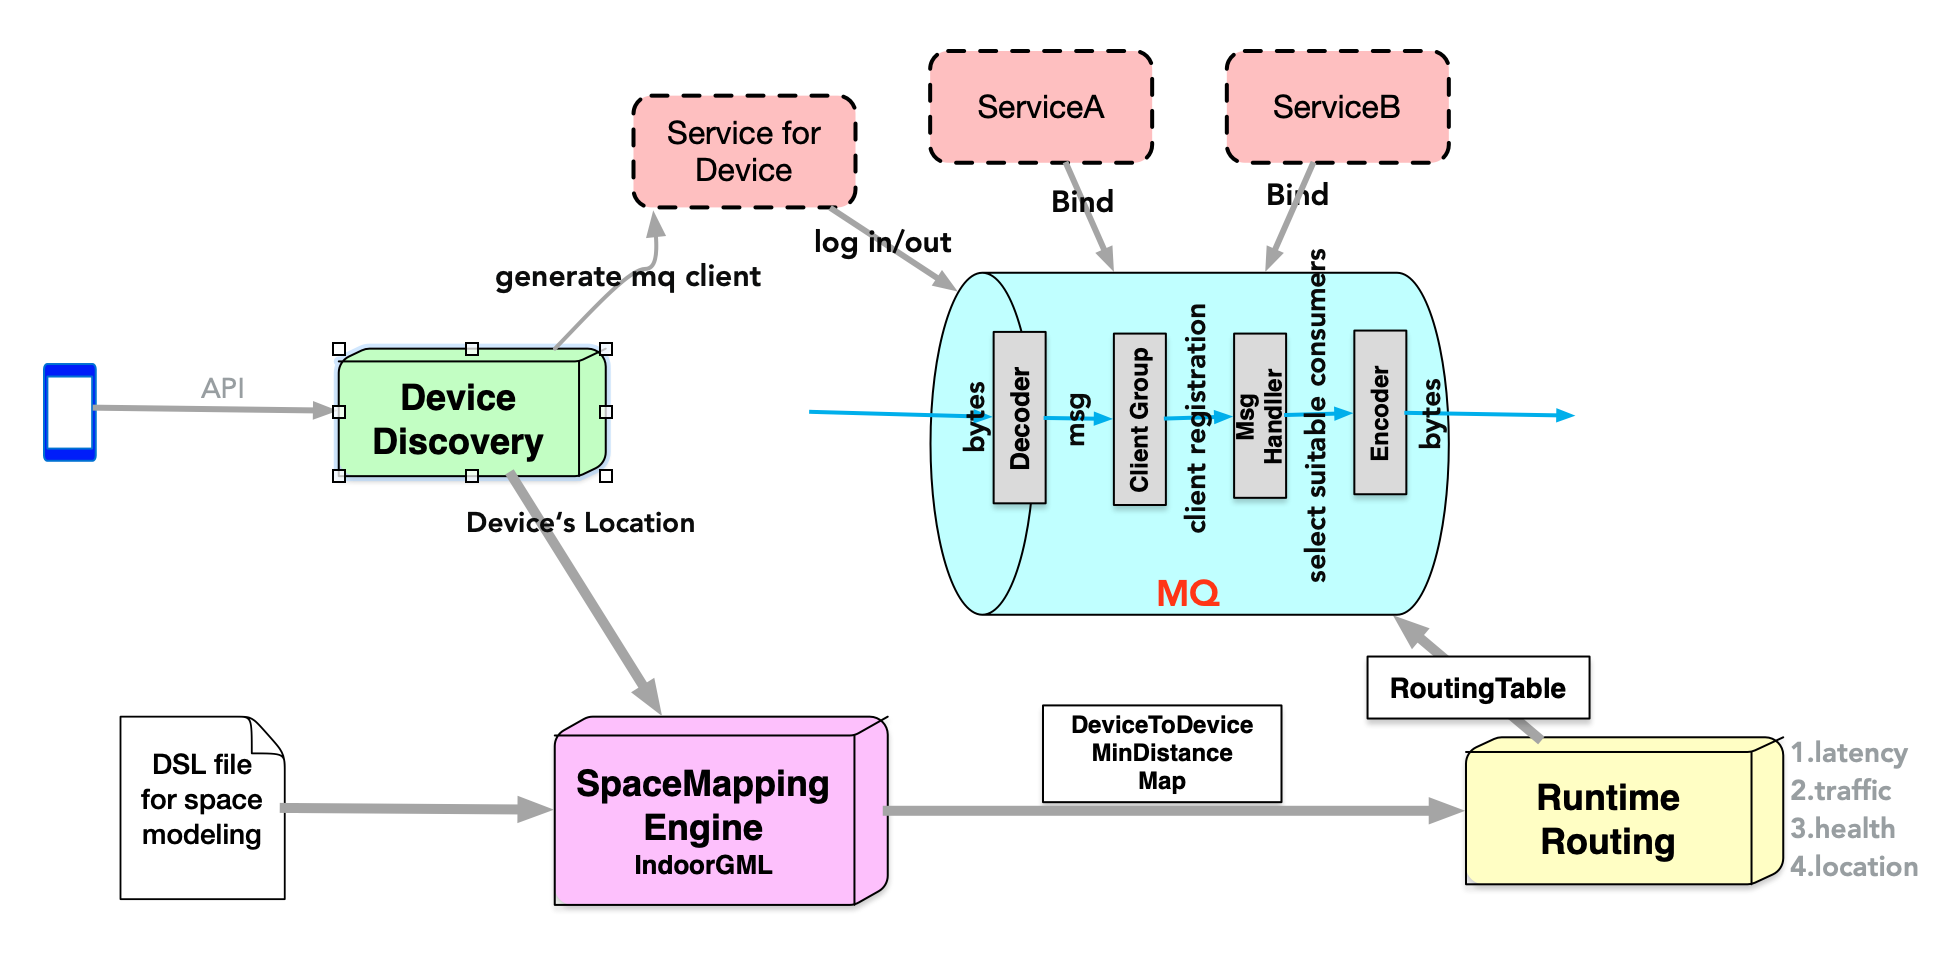
\includegraphics[height=5cm]{images/routing_1.png}
 \caption{消息路由架构图}
 \label{fig:singleblock}
\end{figure}
以"距离最近"策略为例,首先开发人员需要向平台中的空间映射引擎传入一个配置文件来对整个场景进行空间建模,这样空间映射引擎就可以得到整个空间中每个子空间之间的距离信息,当资源服务注册到平台中时,资源服务的位置信息也会被注入到空间映射引擎中去,这样平台就可以得到平台中资源服务之间的距离信息,将距离信息存入一个哈希表中发送给运行路由模块,运行时路由模块中根据开发人员传入的策略信息,会生成不同策略下的路由表,如“就近优先”表,“成本最低”表等,运行时路由模块会定时向消息中间件推送这些路由表,消息中间件中的路由表会定期更新。
//todo
\begin{figure}[ht]
 \centering
 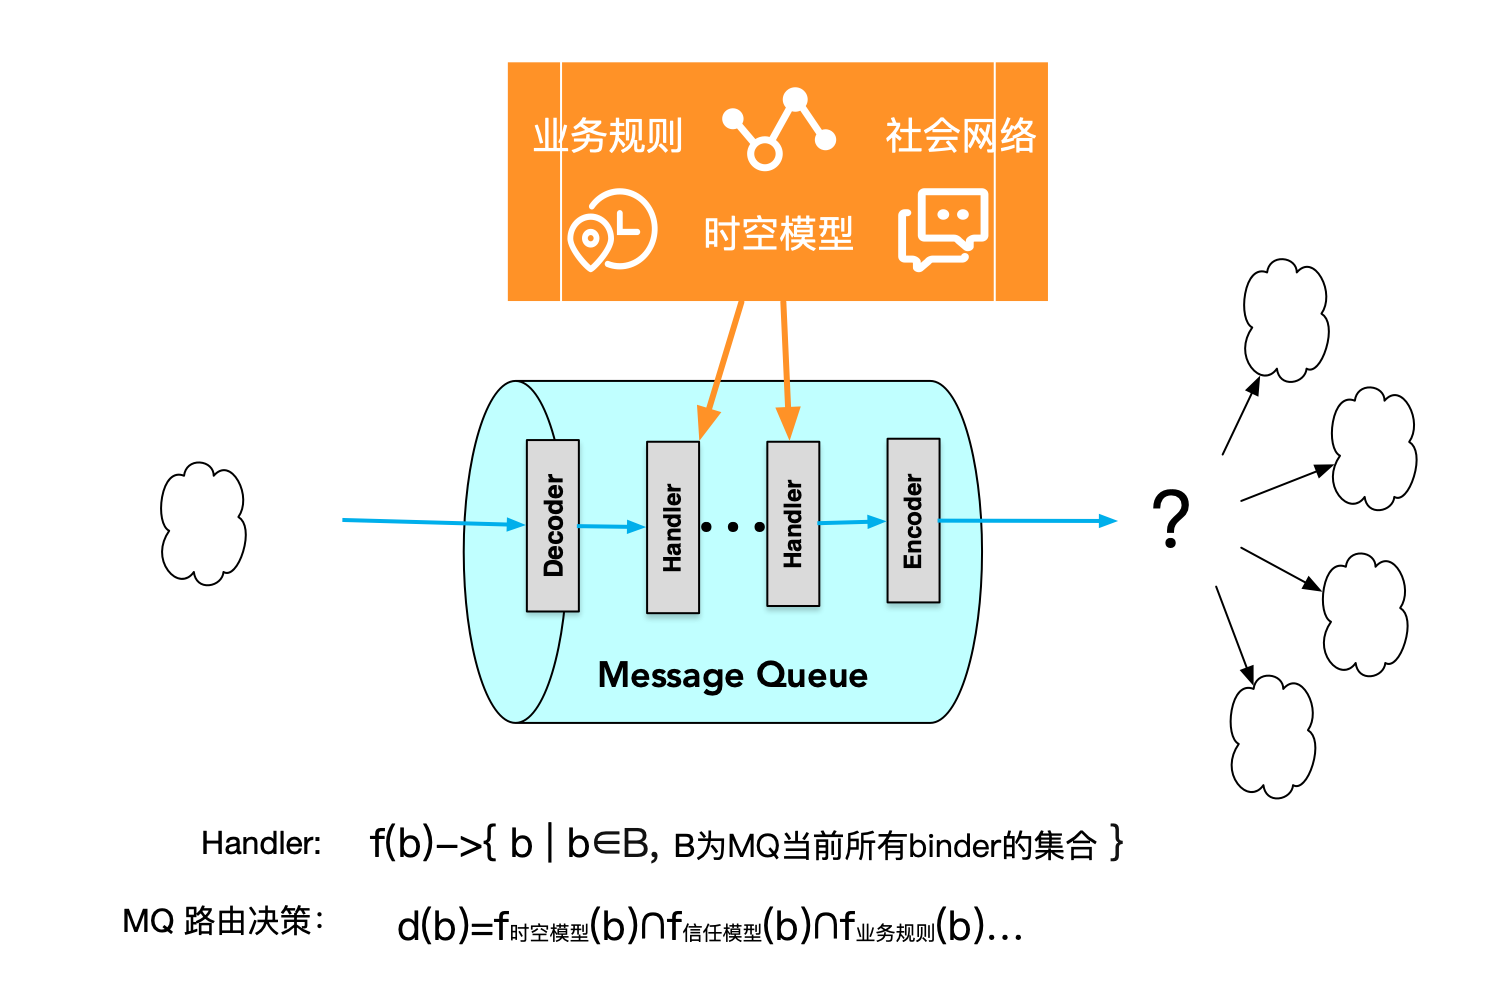
\includegraphics[height=5cm]{images/routing.png}
 \caption{消息路由}
 \label{fig:singleblock}
\end{figure}
\subsubsection{资源服务的动态更新}

\newpage

% -----------------------------------REFERENCE----------------------------------------
\section{引用示例}
This document is an example of BibTeX using in bibliography management. Three items are cited: \textit{The \LaTeX\ Companion} book \cite{latexcompanion}, the Einstein journal paper \cite{einstein}, and the Donald Knuth's website \cite{knuthwebsite}. The \LaTeX\ related items are \cite{latexcompanion,knuthwebsite}. 

% -----------------------------------Appendix----------------------------------------
% -----------------------------------REFERENCE----------------------------------------
\newpage
\bibliographystyle{unsrt}
\bibliography{ReportTemp_ch_xelatex}
\end{document}

